\section{Autonomous Second Order Equations}

\noindent
A second order differential equation that can be written as
\begin{equation} \label{eq:4.4.1}
y''=F(y,y')
\end{equation}
where $F$ is independent of $t$, is said to be {\color{blue}\it autonomous\/}.
An autonomous second order equation can be converted into a first
order equation relating $v=y'$ and $y$. If we let $v=y'$,
\eqref{eq:4.4.1} becomes
\begin{equation} \label{eq:4.4.2}
v'=F(y,v).
\end{equation}
Since
\begin{equation} \label{eq:4.4.3}
v'={dv\over dt}={dv\over dy}{dy\over dt}=v{dv\over dy},
\end{equation}
\eqref{eq:4.4.2} can be rewritten as
\begin{equation} \label{eq:4.4.4}
v{dv\over dy}=F(y,v).
\end{equation}
The integral curves of \eqref{eq:4.4.4} can be plotted in the $(y,v)$
plane, which is called the
\href{https://mathshistory.st-andrews.ac.uk/Biographies/Poincare/}
{\color{blue}\it Poincar\'e
 phase plane\/} of \eqref{eq:4.4.1}. If $y$ is a solution of
\eqref{eq:4.4.1}
then $y=y(t)$, $v=y'(t)$ is a parametric equation for an integral curve
of \eqref{eq:4.4.4}. We'll call these integral curves {\color{blue}\it
trajectories\/} of \eqref{eq:4.4.1}, and we'll call
\eqref{eq:4.4.4} the {\color{blue}\it phase plane equivalent\/} of \eqref{eq:4.4.1}.

In this section we'll consider  autonomous equations
that can be written as
\begin{equation} \label{eq:4.4.5}
y''+q(y,y')y'+p(y)=0.
\end{equation}
Equations of this form often arise in applications of Newton's second
law of motion. For example, suppose  $y$ is the displacement of a
moving object with mass $m$. It's  reasonable to think of two
types of time-independent forces acting on the object. One type - such
as gravity - depends only on position. We could write such a force as
$-mp(y)$. The second type - such as atmospheric resistance or friction
- may depend on position and velocity. (Forces that depend on velocity
are called {\color{blue}\it damping\/} forces.) We  write this force as
$-mq(y,y')y'$, where $q(y,y')$ is usually a positive function and
we've put the factor $y'$ outside  to make it
explicit that the force
is in the direction opposing the motion. In this case Newton's, second
law of motion leads to \eqref{eq:4.4.5}.

The phase plane equivalent of \eqref{eq:4.4.5} is
\begin{equation} \label{eq:4.4.6}
v{dv\over dy}+q(y,v)v+p(y)=0.
\end{equation}
Some  statements that we'll be making about the properties of
\eqref{eq:4.4.5} and \eqref{eq:4.4.6} are intuitively reasonable, but
difficult to prove.
Therefore our presentation in this section will be informal: we'll
just say things without proof, all of which are true if we assume that
$p=p(y)$ is continuously differentiable for all $y$ and $q=q(y,v)$ is
continuously differentiable for all $(y,v)$.
 We begin with the following statements:

\begin{itemize}
\item{\bf Statement 1.} If $y_0$ and $v_0$ are arbitrary real numbers then
\eqref{eq:4.4.5} has a unique solution on $(-\infty,\infty)$ such that
$y(0)=y_0$ and $y'(0)=v_0$.

\item{\bf Statement 2.)} If $y=y(t)$ is a solution of \eqref{eq:4.4.5}
and
$\tau$ is any constant then $y_1=y(t-\tau)$ is also a solution of
\eqref{eq:4.4.5}, and $y$ and $y_1$ have the same trajectory.

\item{\bf Statement 3.}   If two solutions $y$ and $y_1$ of
\eqref{eq:4.4.5} have the same trajectory then  $y_1(t)=y(t-\tau)$
for some constant $\tau$.

\item{\bf Statement 4.} Distinct trajectories of \eqref{eq:4.4.5} can't
intersect; that is, if two trajectories of \eqref{eq:4.4.5}
intersect,  they are identical.

\item{\bf Statement 5.} If the trajectory of a solution of
\eqref{eq:4.4.5}
is a closed curve then  $(y(t),v(t))$ traverses the
trajectory in a finite time $T$, and the solution is periodic with
period $T$; that is, $y(t+T)=y(t)$ for all $t$ in $(-\infty,\infty)$.
\end{itemize}

If $\overline y$ is a constant such that $p(\overline y)=0$ then
$y\equiv\overline y$ is a constant solution of \eqref{eq:4.4.5}. We say
that $\overline y$ is an {\color{blue}\it equilibrium\/} of \eqref{eq:4.4.5} and
 $(\overline y,0)$ is a {\color{blue}\it critical point\/} of the phase plane
equivalent equation \eqref{eq:4.4.6}. We say that the equilibrium and
the critical point are {\color{blue}\it stable\/} if, for any given $\epsilon>0$
{\color{blue}\it no matter how small\/}, there's a $\delta>0$,
{\color{blue}\it
sufficiently small\/}, such that if
$$
\sqrt{(y_0-\overline y)^2+v_0^2}<\delta
$$
then the  solution of the initial value problem
$$
y''+q(y,y')y'+p(y)=0,\quad y(0)=y_0,\quad y'(0)=v_0
$$
satisfies the inequality
$$
\sqrt{(y(t)-\overline y)^2+(v(t))^2}<\epsilon
$$
for all $t>0$. Figure~\ref{figure:4.4.1} illustrates the geometrical
interpretation of this definition in the Poincar\'e phase plane: if
$(y_0,v_0)$ is in the smaller shaded circle (with radius~$\delta$), then
$(y(t),v(t))$ must be in the larger circle (with
radius~$\epsilon$) for all $t>0$.

\begin{figure}[H]
  \centering
  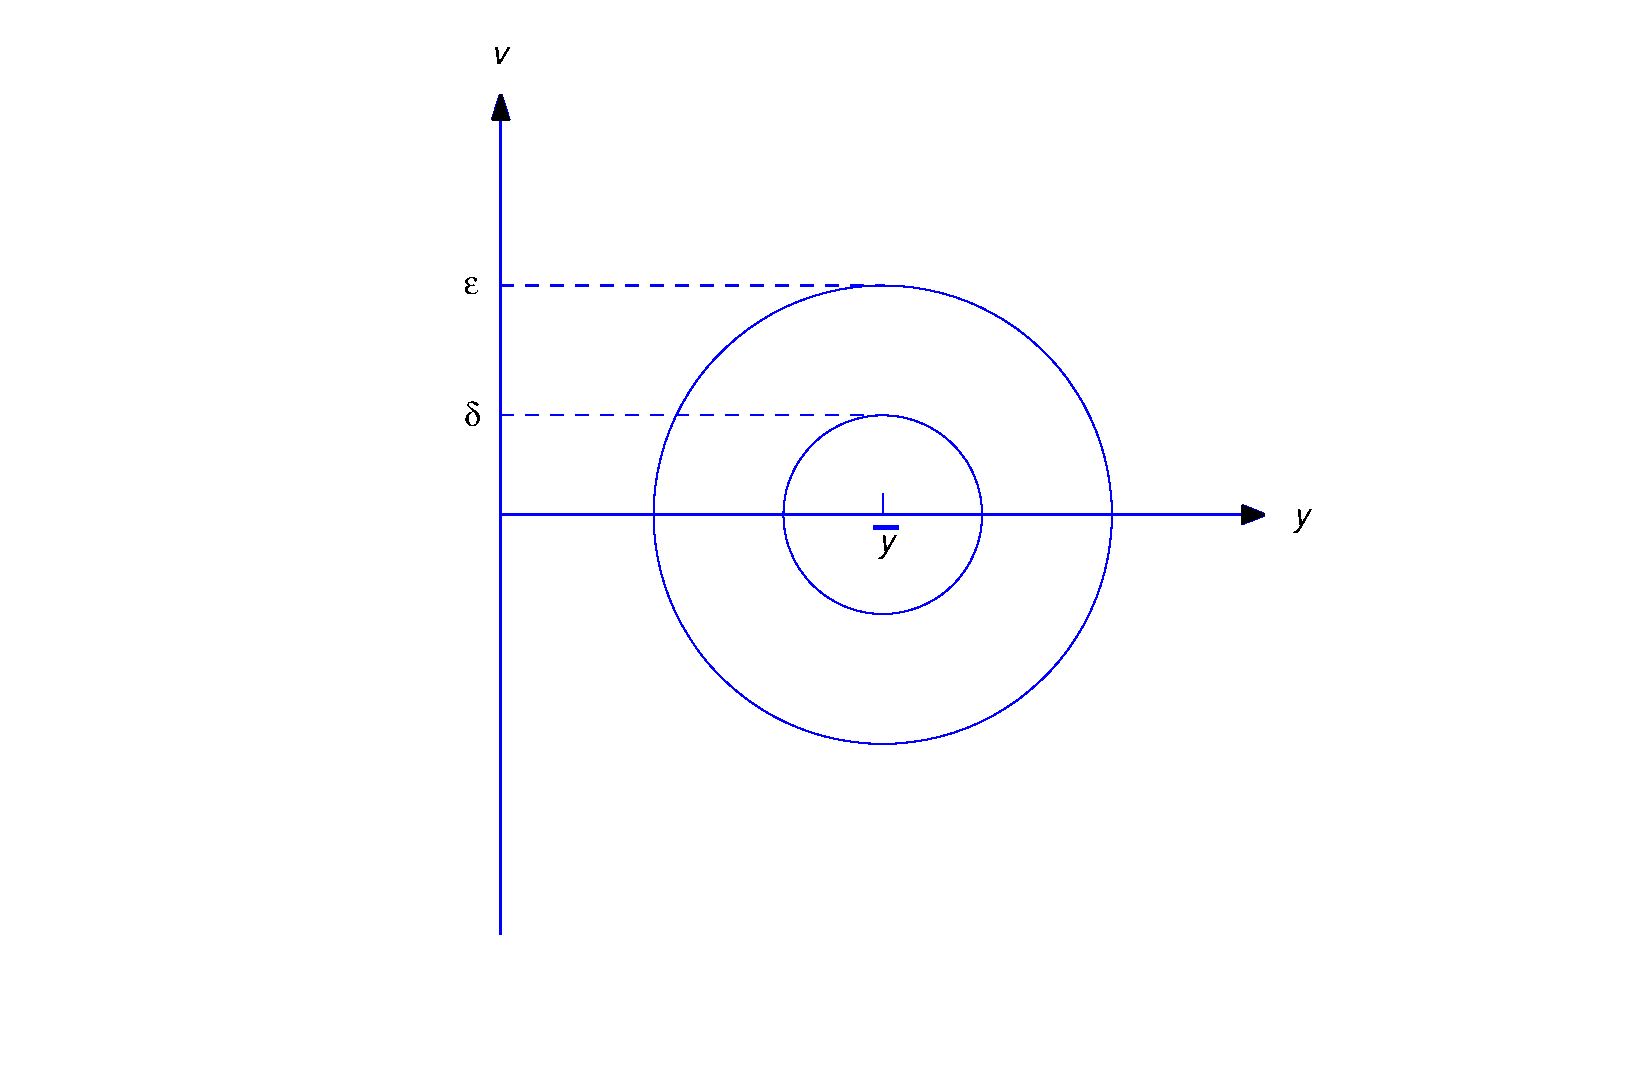
\includegraphics[bb=-78 148 689 643,width=5.67in,height=3.66in,keepaspectratio]{fig040401}
\color{blue}
\caption{Stability: if $(y_0,v_0)$ is in the smaller
circle  then $(y(t),v(t))$ is in the larger circle for all $t>0$}
  \label{figure:4.4.1}
\end{figure}

If an equilibrium and the associated critical point are not stable, we
say they are {\color{blue}\it unstable\/}. To see if you really understand what
{\color{blue}\it stable\/} means, try to give a direct definition of {\color{blue}\it
unstable\/}
(Exercise~\ref{exer:4.4.22}). We'll illustrate both definitions in
the following examples.

\boxit{The Undamped Case}

\noindent
We'll begin with the case where $q\equiv0$, so  \eqref{eq:4.4.5}
reduces to
 \begin{equation} \label{eq:4.4.7}
y''+p(y)=0.
\end{equation}
We say that this equation - as well as any physical situation
that it may model - is {\color{blue}\it undamped\/}.
The phase plane equivalent of \eqref{eq:4.4.7} is  the
separable equation
$$
v{dv\over dy}+p(y)=0.
$$
 Integrating this  yields
\begin{equation} \label{eq:4.4.8}
{v^2\over2}+P(y)=c,
\end{equation}
where $c$ is a constant of integration and $P(y)=\int p(y)\,dy$ is an
antiderivative of $p$.

If \eqref{eq:4.4.7} is the equation of motion of an object of
mass $m$, then
 $mv^2/2$ is the kinetic energy and $mP(y)$ is the
potential energy of the object;   thus, \eqref{eq:4.4.8} says that the
total
energy of the object remains constant, or is {\color{blue}\it conserved\/}. In
particular, if a trajectory passes through a given point $(y_0,v_0)$
then
$$
c={v_0^2\over2}+P(y_0).
$$

\begin{example}$[$The Undamped Spring - Mass
System$]\,$\label{example:4.4.1}\rm
 Consider an object with mass $m$ suspended from a
spring and moving vertically. Let $y$ be the displacement of the
object from the position it occupies when suspended at rest from the
spring (Figure~\ref{figure:4.4.2}).

\begin{figure}[H]
  \centering
  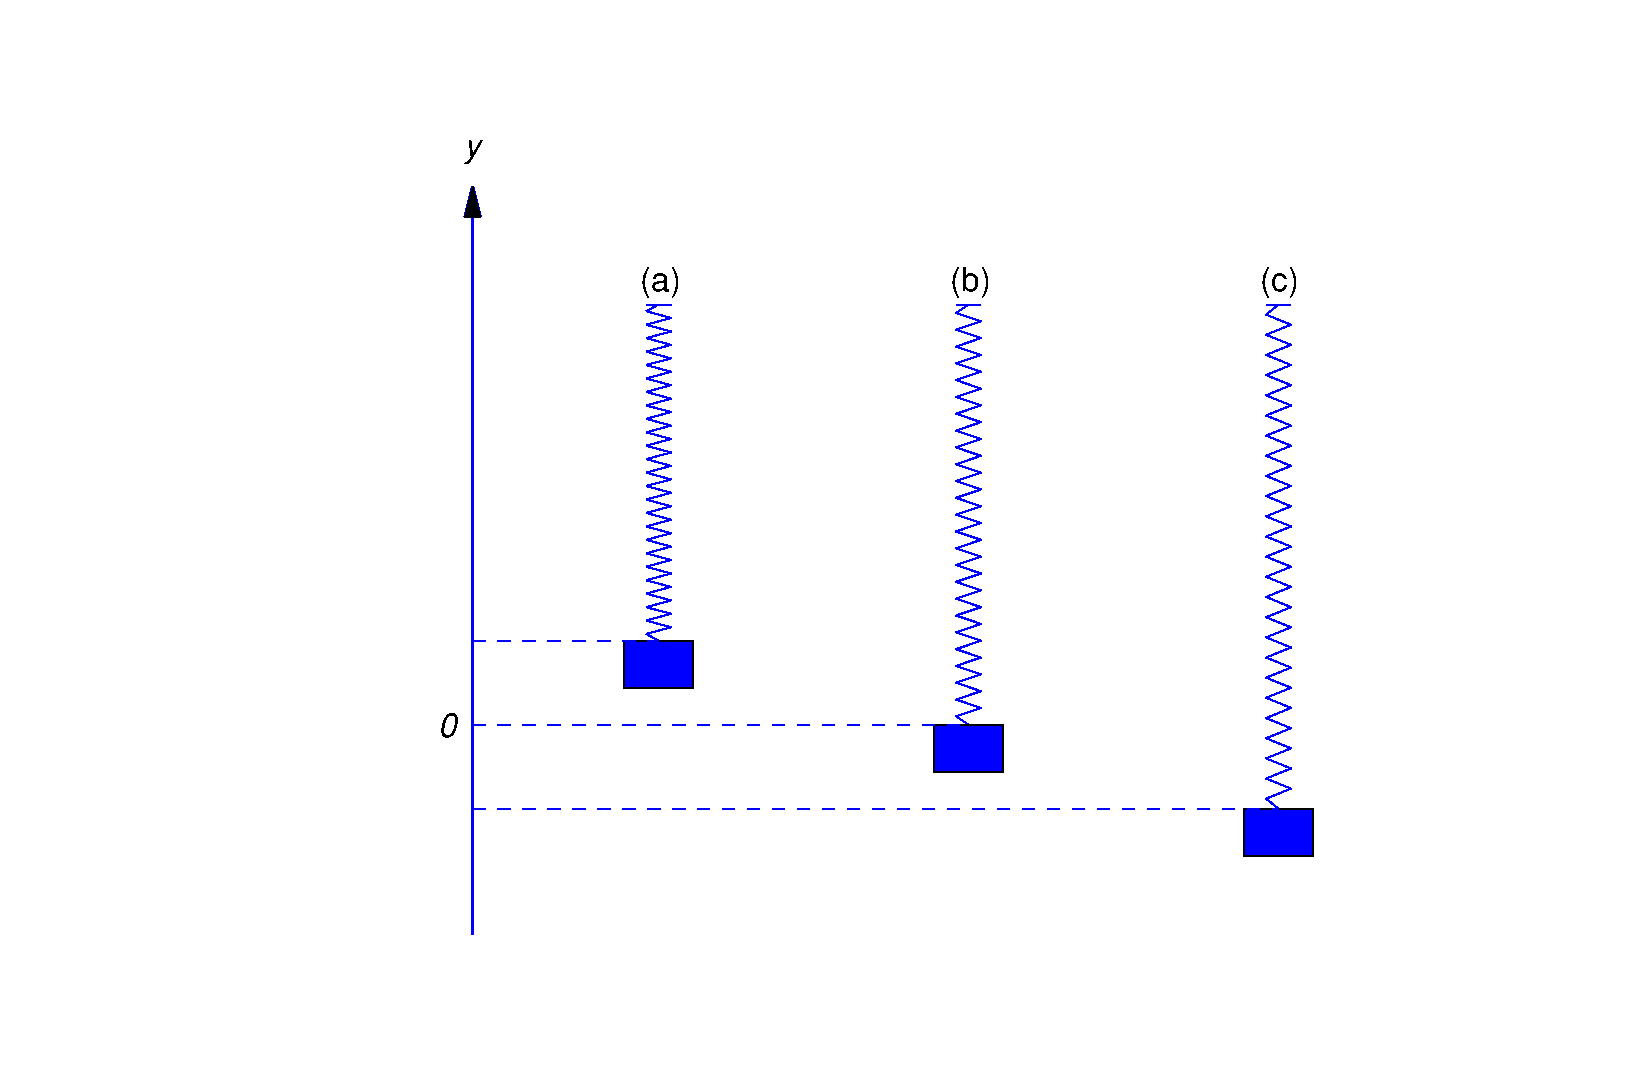
\includegraphics[bb=-78 148 689 643,width=5.67in,height=3.66in,keepaspectratio]{fig040402}
\color{blue}
  \caption{\,\part{a}  $y>0$   \, \part{b}  $y=0$   \, \part{c}  $y<0$}
  \label{figure:4.4.2}
\end{figure}

Assume that if the length of the spring is changed by an amount
$\Delta L$ (positive or negative), then the spring exerts an opposing
force with magnitude $k|\Delta L|$, where k is a positive constant. In
Section~6.1 it will be shown that if the mass of the spring
is negligible compared to $m$ and no other forces act on the object then
Newton's second law of motion implies that
\begin{equation} \label{eq:4.4.9}
my''=-ky,
\end{equation}
which can be written in the form \eqref{eq:4.4.7} with $p(y)=ky/m$. This
equation can be solved easily by a method that we'll study in
Section~5.2, but that method isn't available here. Instead,
we'll consider the phase plane equivalent of \eqref{eq:4.4.9}.

From \eqref{eq:4.4.3}, we can rewrite \eqref{eq:4.4.9} as the separable
equation
$$
 mv{dv\over dy}=-ky.
$$
Integrating this  yields
$$
{mv^2\over2}=-{ky^2\over2}+c,
$$
which implies that
\begin{equation} \label{eq:4.4.10}
mv^2+ky^2=\rho
\end{equation}
($\rho=2c$). This defines an ellipse in the Poincar\'e phase plane
(Figure~\ref{figure:4.4.3}).

\begin{figure}[tbp]
  \centering
  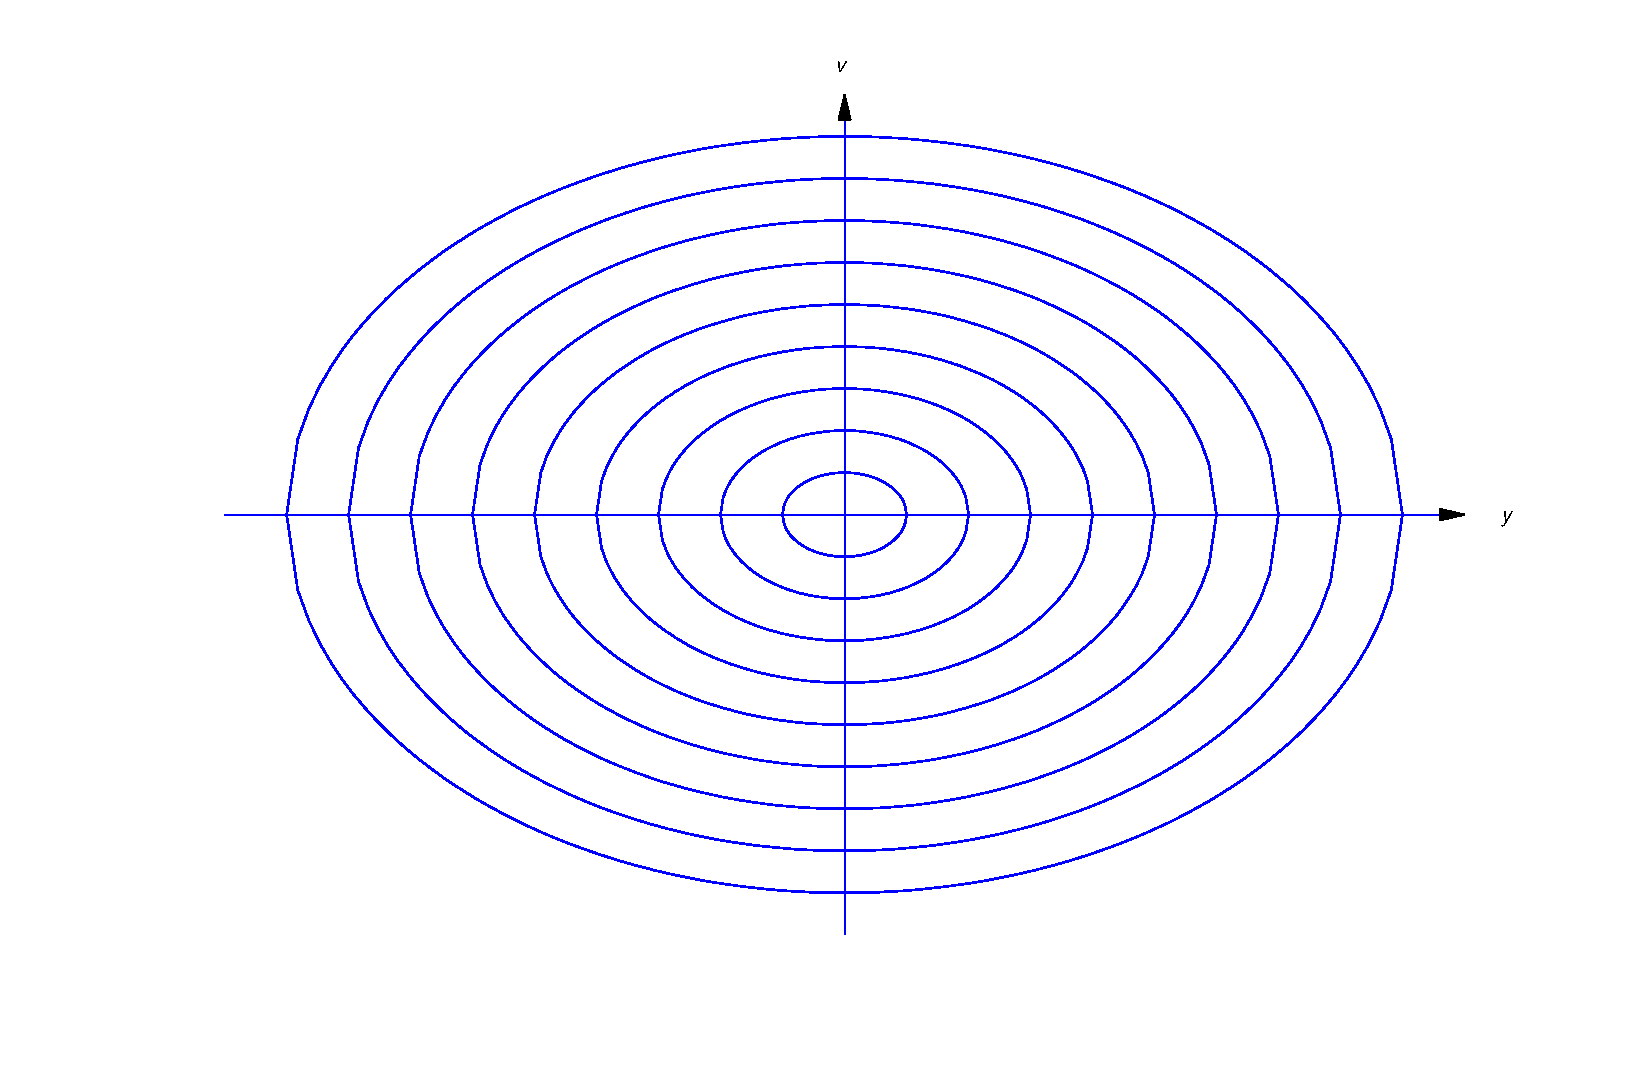
\includegraphics[bb=-78 148 689 643,width=5.67in,height=3.66in,keepaspectratio]{fig040403}
\color{blue}
\caption{Trajectories of  $my''+ky=0$}
  \label{figure:4.4.3}
\end{figure}

We can identify $\rho$ by setting $t=0$ in \eqref{eq:4.4.10};   thus,
$\rho=mv_0^2+ky_0^2$, where $y_0=y(0)$ and $v_0=v(0)$. To determine
the maximum and minimum values of $y$ we set $v=0$ in \eqref{eq:4.4.10};
thus,
\begin{equation} \label{eq:4.4.11}
y_{\max}=R\mbox{\quad and \quad}
y_{\min}=-R,\mbox{\quad with } R=\sqrt{\rho\over k}.
\end{equation}
Equation~\eqref{eq:4.4.9} has exactly one equilibrium, $\overline y=0$,
and
it's stable. You can see intuitively why this is so: if the object is
displaced in either direction from  equilibrium, the spring tries
to bring it back.

In this case we can find $y$ explicitly as a function of $t$. (Don't
expect this to happen in more complicated problems!) If $v>0$ on an
interval $I$,  \eqref{eq:4.4.10} implies that
$$
{dy\over dt}=v=\sqrt{\rho-ky^2\over m}
$$
on $I$. This is equivalent to
\begin{equation} \label{eq:4.4.12}
{\sqrt k\over\sqrt{\rho-ky^2}}{dy\over dt}=\omega_0,\mbox{\quad where
\quad}
\omega_0=\sqrt{k\over m}.
\end{equation}
Since
$$
\int{\sqrt k\,dy\over\sqrt{\rho-ky^2}}=\sin^{-1}\left(\sqrt{k\over\rho
}y\right)+c=\sin^{-1}\left(y\over R\right)+c
$$
(see \eqref{eq:4.4.11}), \eqref{eq:4.4.12} implies that that there's a
constant $\phi$ such that
$$
\sin^{-1}\left(y\over R\right)=\omega_0 t+\phi
$$
or
$$
y=R\sin(\omega_0 t+\phi)
$$
for all $t$ in $I$. Although we obtained this function by assuming that
$v>0$, you can easily verify that $y$ satisfies \eqref{eq:4.4.9} for all
values of $t$. Thus, the displacement varies periodically between $-R$
and $R$, with period $T=2\pi/\omega_0$ (Figure~\ref{figure:4.4.4}). (If
you've taken a course in elementary mechanics you may recognize this
as {\color{blue}\it simple harmonic motion\/}.)
\end{example}

\begin{figure}[tbp]
  \centering
  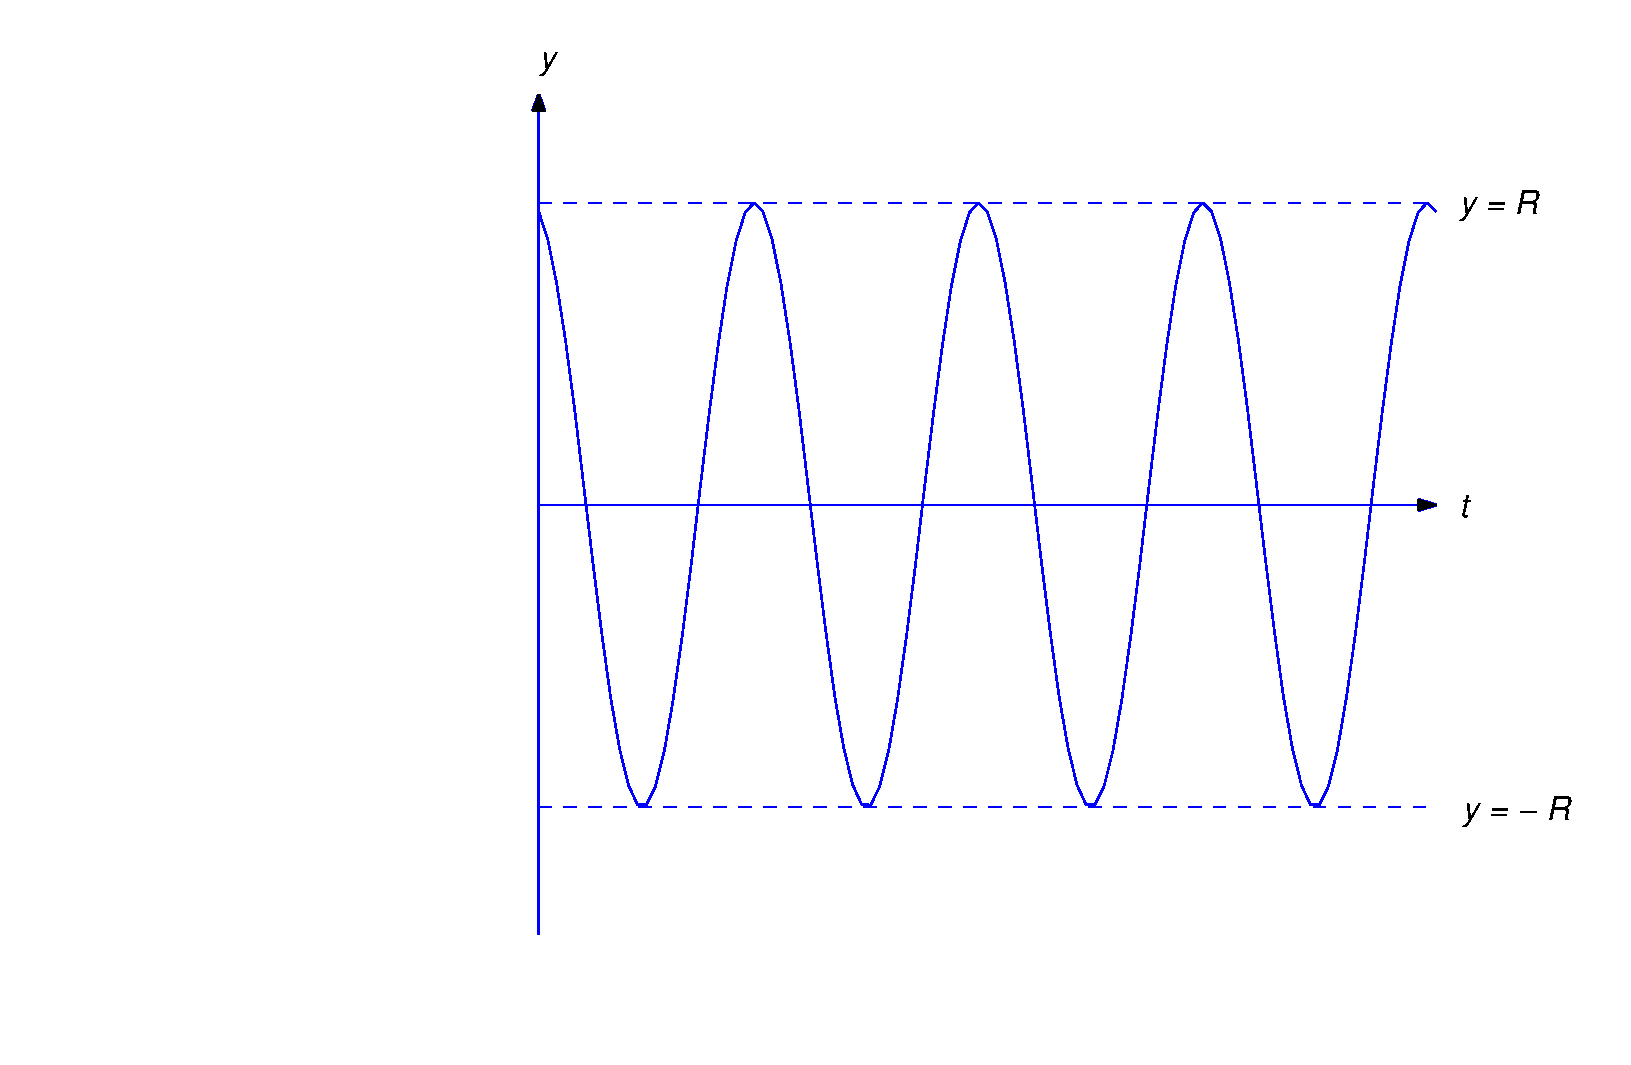
\includegraphics[bb=-78 148 689 643,width=5.67in,height=3.66in,keepaspectratio]{fig040404}
\color{blue}
\caption{$y=R\sin(\omega_0 t+\phi)$}
  \label{figure:4.4.4}
\end{figure}

\begin{example}$[$The Undamped Pendulum$]$\label{example:4.4.2}\rm
\, Now we
consider the motion of a pendulum with mass $m$, attached to the end
of a weightless rod with length $L$ that rotates on a frictionless
axle (Figure~\ref{figure:4.4.5}). We assume that there's no air
resistance.

Let $y$ be the angle measured from the rest position
(vertically downward) of the pendulum, as shown in
Figure~\ref{figure:4.4.5}. Newton's second law of motion says that the
product of $m$ and the tangential acceleration equals the tangential
component of the gravitational force;  therefore, from
Figure~\ref{figure:4.4.5},
$$
mLy''=-mg\sin y,
$$
or
\begin{equation} \label{eq:4.4.13}
y''=-{g\over L} \sin y.
\end{equation}

\begin{figure}[tbp]
  \centering
\scalebox{.5}{
  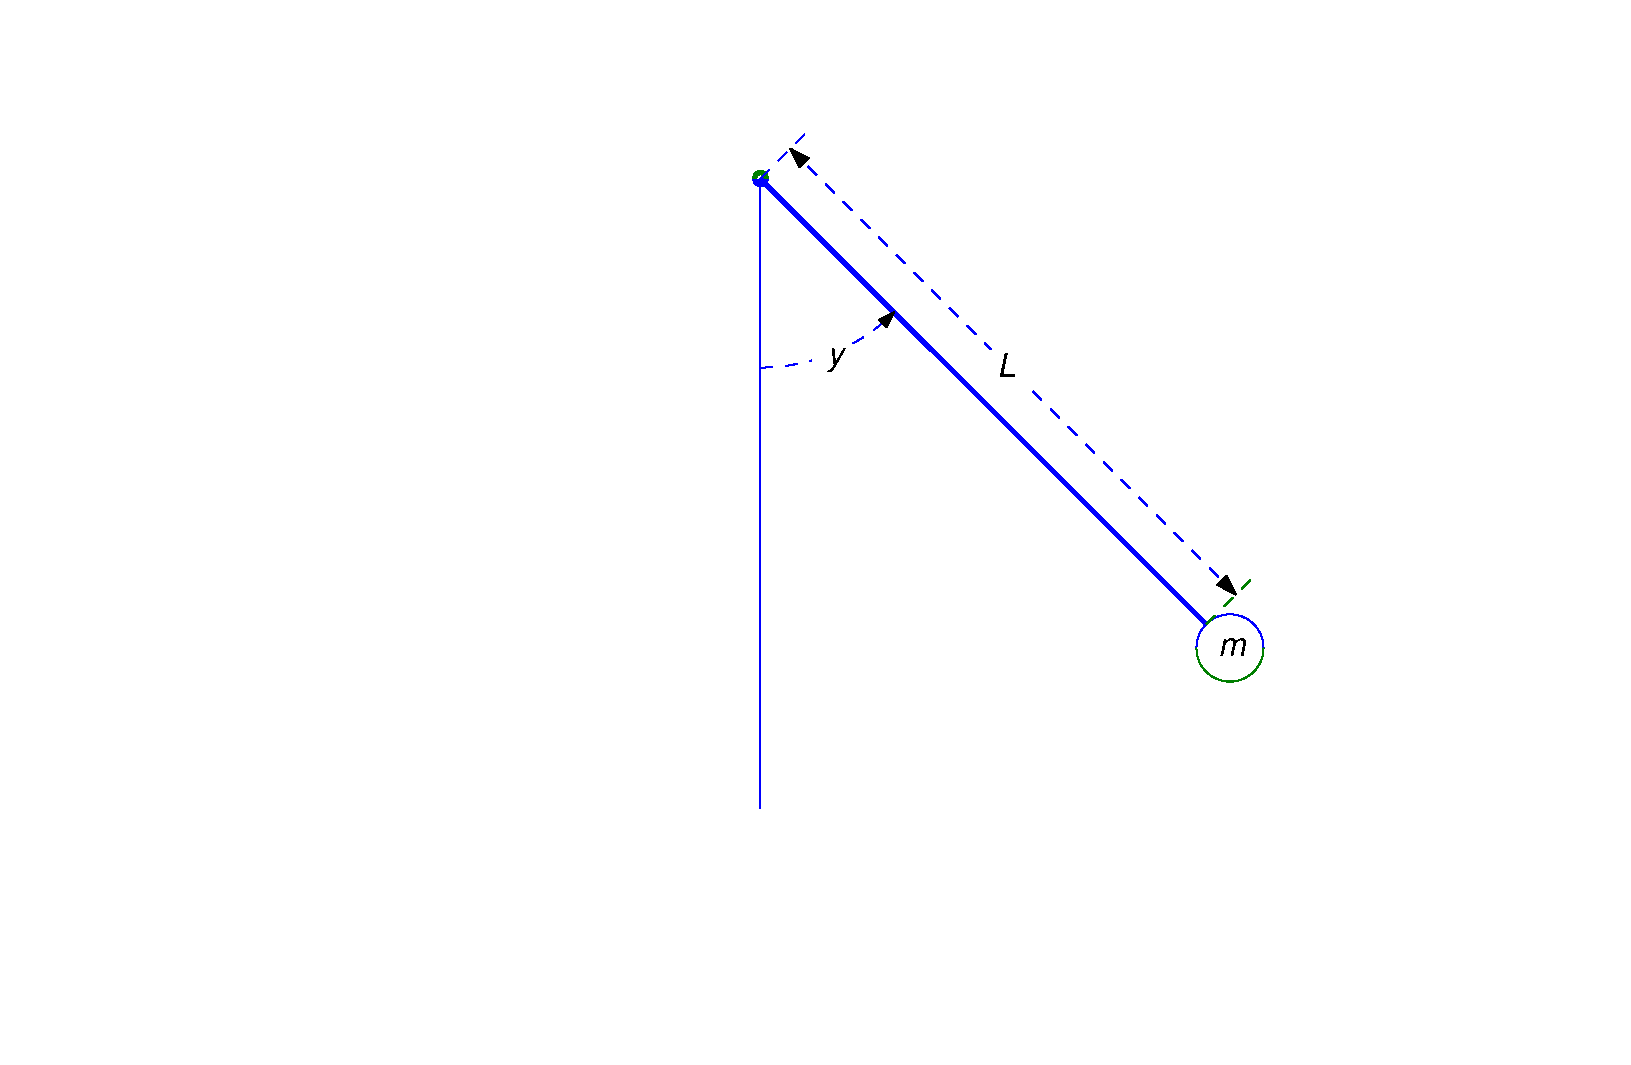
\includegraphics[bb=-78 148 689 643,width=5.67in,height=3.66in,keepaspectratio]{fig040405} }
\color{blue}
\caption{ The undamped pendulum}
  \label{figure:4.4.5}
\end{figure}

Since $\sin n\pi=0$ if $n$ is any integer,  \eqref{eq:4.4.13} has
infinitely many equilibria $\overline y_n=n\pi$. If $n$ is
even, the mass is directly below the axle
(Figure~\ref{figure:4.4.6}~\part{a}) and gravity opposes any deviation
from the equilibrium. However, if $n$ is odd, the mass is directly
above the axle (Figure~\ref{figure:4.4.6}~\part{b}) and gravity
increases any deviation from the equilibrium. Therefore we conclude
on physical grounds that $\overline y_{2m}=2m\pi$ is stable and
$\overline y_{2m+1}=(2m+1)\pi$ is unstable.

\begin{figure}[tbp]
  \centering
\scalebox{.5}{
  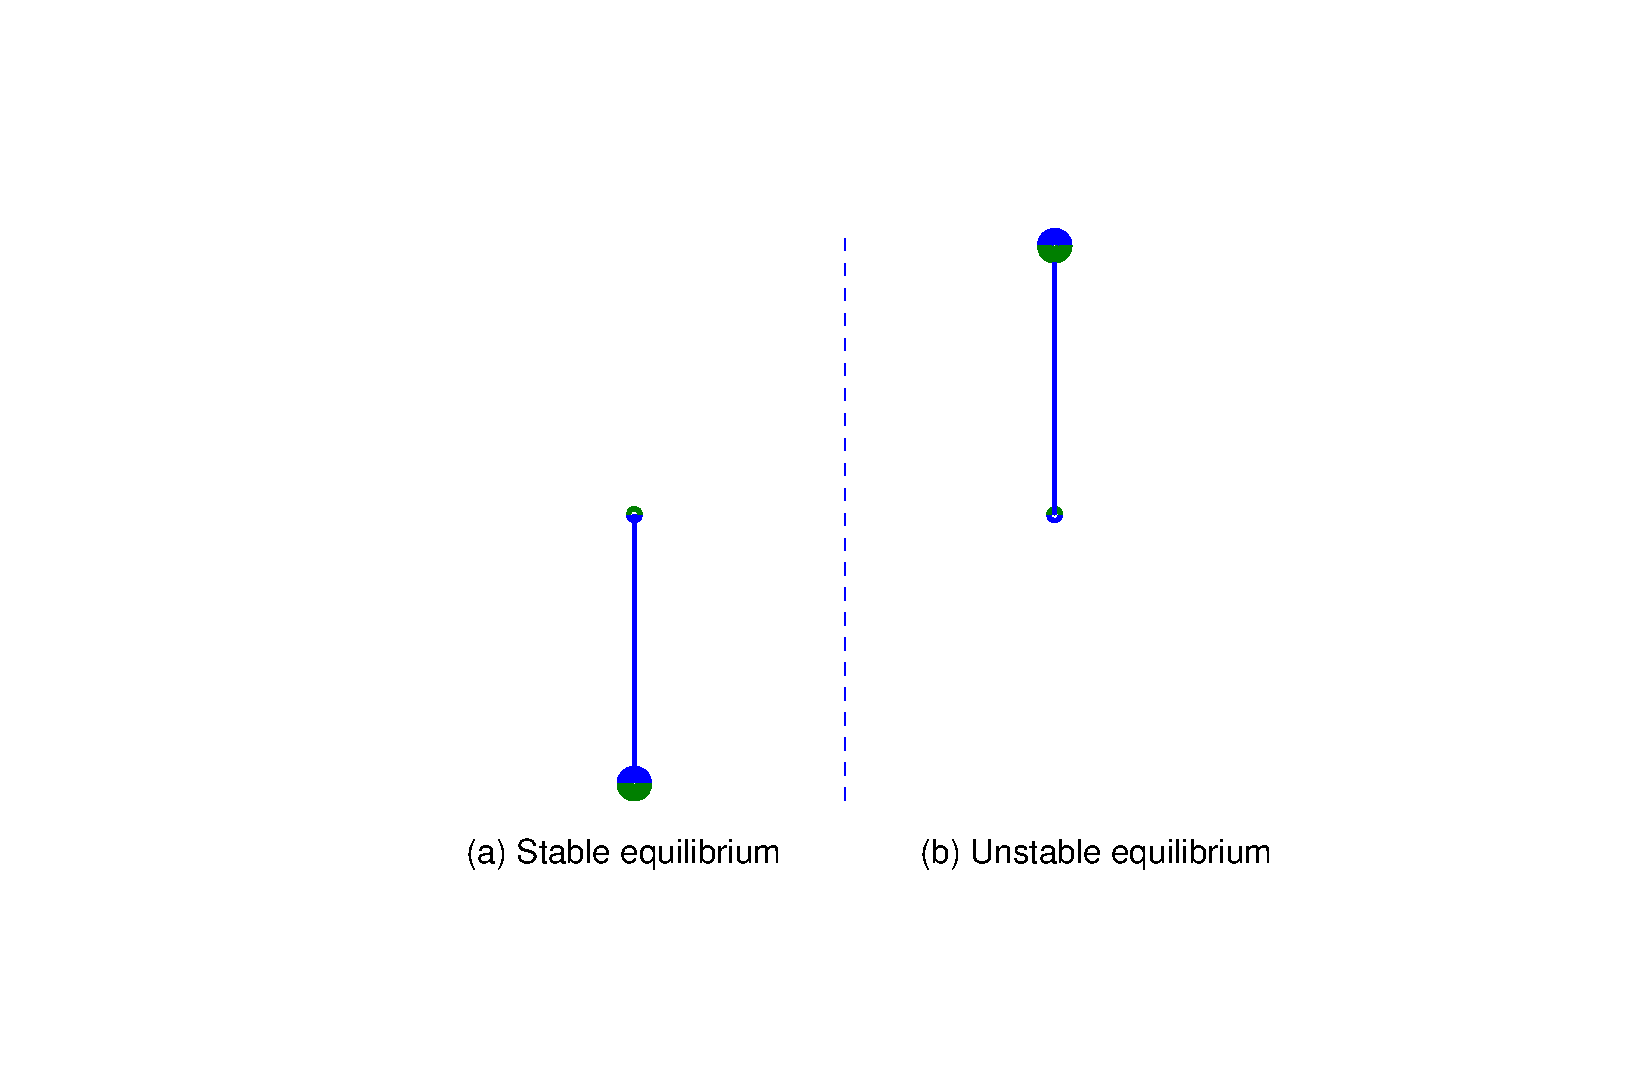
\includegraphics[bb=-78 148 689 643,width=5.67in,height=3.66in,keepaspectratio]{fig040406} }
\color{blue}
\caption{ \part{a}\, Stable equilibrium  \, \part{b}\, Unstable
equilibrium}
  \label{figure:4.4.6}
\end{figure}

The phase plane equivalent of \eqref{eq:4.4.13} is
$$
v{dv\over dy}=-{g\over L}\sin y,
$$
where $v=y'$ is the angular velocity of the pendulum. Integrating this
yields
\begin{equation} \label{eq:4.4.14}
{v^2\over2}={g\over L}\cos y+c.
\end{equation}
If $v=v_0$ when $y=0$, then
$$
c={v_0^2\over2}-{g\over L},
$$
so \eqref{eq:4.4.14} becomes
$$
{v^2\over2}={v_0^2\over2}-{g\over L}(1-\cos y)
={v_0^2\over2}-{2g\over L}\sin^2{y\over2},
$$
which is equivalent to
\begin{equation} \label{eq:4.4.15}
v^2=v_0^2-v_c^2\sin^2{y\over2},
\end{equation}
 where
$$
v_c=2\sqrt{g\over L}.
$$

The curves defined by \eqref{eq:4.4.15} are the trajectories of
\eqref{eq:4.4.13}. They are periodic with period $2\pi$ in $y$, which isn't
 surprising, since if $y=y(t)$ is a solution of \eqref{eq:4.4.13} then
so is $y_n=y(t)+2n\pi$ for any integer $n$. Figure~\ref{figure:4.4.7}
shows trajectories over the interval $[-\pi,\pi]$. From \eqref{eq:4.4.15},
you can see that if $|v_0|>v_c$ then $v$ is nonzero for all $t$, which
means that the object whirls in the same direction forever, as in
Figure~\ref{figure:4.4.8}. The trajectories associated with this
whirling motion are above the upper dashed curve and below the lower
dashed curve in Figure~\ref{figure:4.4.7}. You can also see from
\eqref{eq:4.4.15} that if $0<|v_0|<v_c$,then $v=0$ when $y=\pm y_{\max}$,
where
$$
y_{\max}=2\sin^{-1}(|v_0|/v_c).
$$
In this case the pendulum oscillates periodically between $-y_{\max}$
and $y_{\max}$, as shown in Figure~\ref{figure:4.4.9}. The
trajectories associated with this kind of motion are the ovals between
the dashed curves in Figure~\ref{figure:4.4.7}. It can be shown (see
Exercise~\ref{exer:4.4.21} for a partial proof) that the period of the
oscillation is
\begin{equation} \label{eq:4.4.16}
T=8\int_0^{\pi/2}{d\theta\over\sqrt{v_c^2-v_0^2\sin^2\theta}}.
\end{equation}
Although this integral can't be evaluated in terms of familiar
elementary functions, you can see that it's finite if $|v_0|<v_c$.

The dashed curves in Figure~\ref{figure:4.4.7} contain four
trajectories. The critical points $(\pi,0)$ and $(-\pi,0)$ are the
trajectories of the unstable equilibrium solutions $\overline
y=\pm\pi$.
The upper dashed curve connecting (but not including) them is obtained
from initial conditions of the form $y(t_0)=0$, $v(t_0)=v_c$. If $y$ is
any solution with this trajectory then
$$
\lim_{t\to\infty}y(t)=\pi\mbox{\quad and \quad}\lim_{t\to-\infty}y(t)=-\pi.
$$
The lower dashed curve connecting (but not including) them is obtained
from initial conditions of the form $y(t_0)=0$, $v(t_0)=-v_c$. If $y$
is any solution with this trajectory then
$$
\lim_{t\to\infty}y(t)=-\pi\mbox{\quad and \quad}\lim_{t\to-\infty}y(t)=\pi.
$$
Consistent with this, the integral \eqref{eq:4.4.16} diverges to $\infty$
if $v_0=\pm v_c$. (Exercise~\ref{exer:4.4.21}) .

Since the dashed curves separate trajectories of whirling solutions
from trajectories of oscillating solutions, each of these curves is
called a {\color{blue}\it separatrix\/}.

In general, if \eqref{eq:4.4.7} has both stable and unstable equilibria
then the separatrices are the curves given by \eqref{eq:4.4.8} that pass
through unstable critical points. Thus, if $(\overline y,0)$ is an
unstable critical point, then
\begin{equation} \label{eq:4.4.17}
{v^2\over 2}+P(y)=P(\overline y)
\end{equation}
\enlargethispage{30pt}
defines a separatrix passing through $(\overline y,0)$.
\end{example}

\newpage
\vspace*{-.2in}
\begin{figure}[H]
  \centering
\scalebox{.5}{
  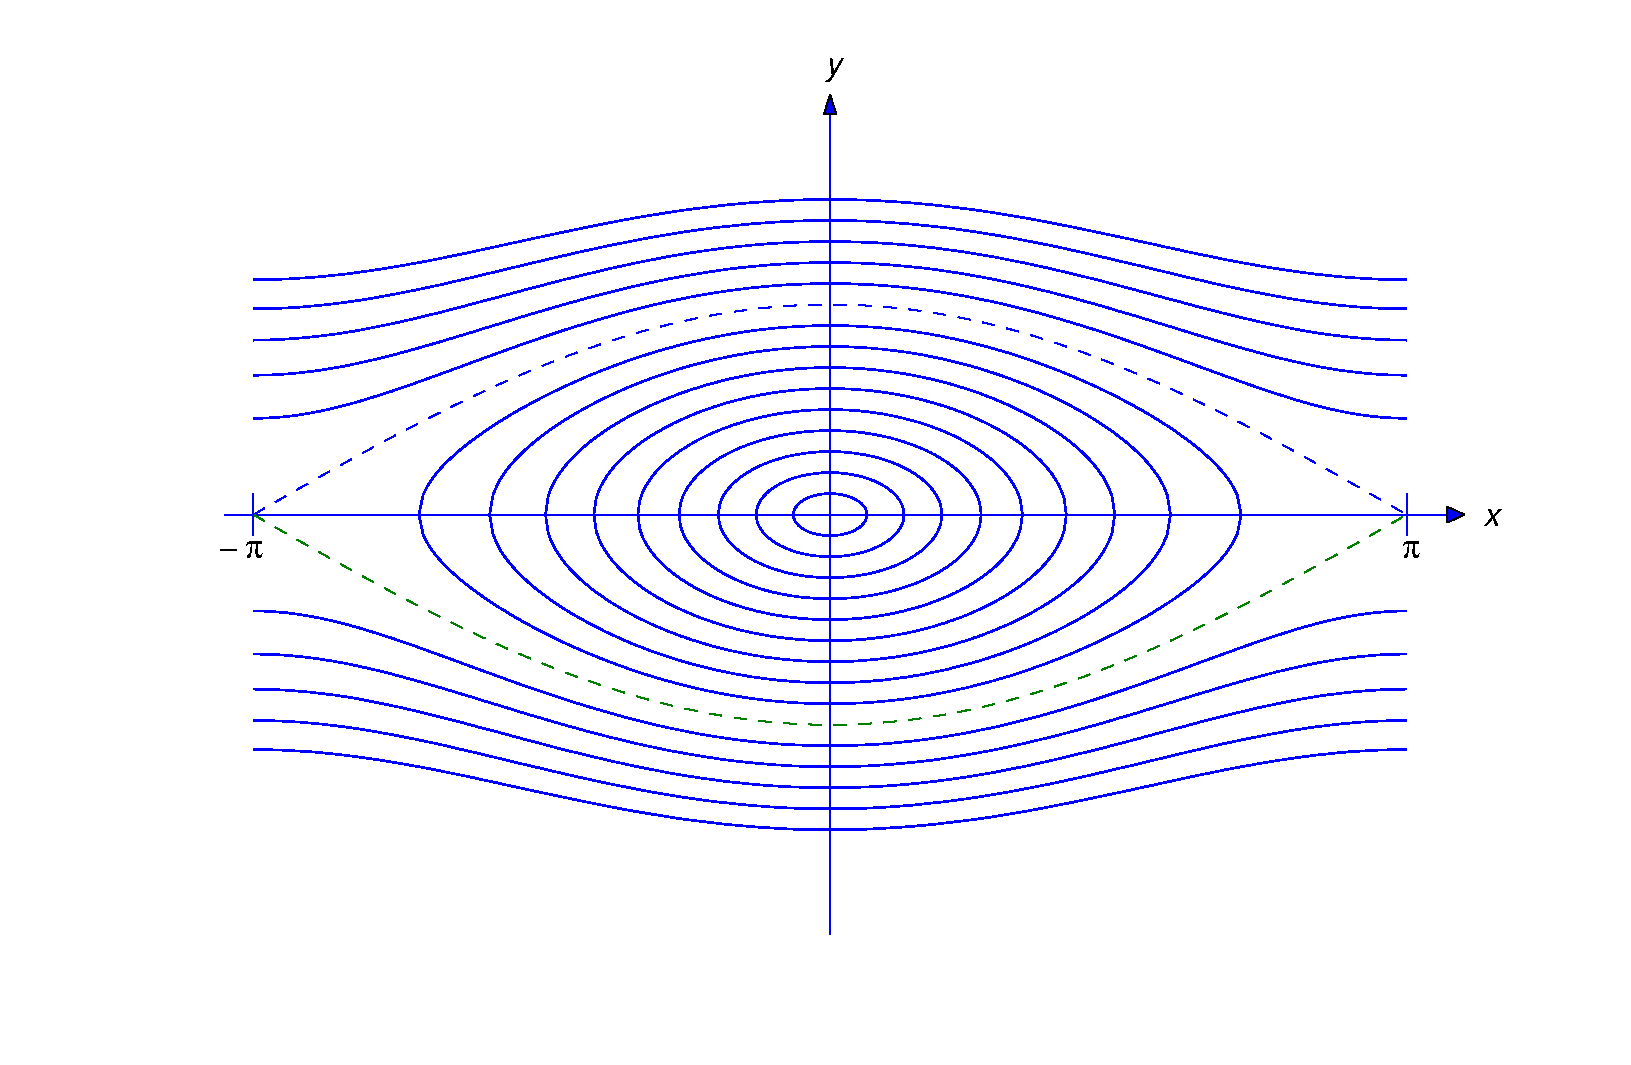
\includegraphics[bb=-78 148 689 643,width=5.67in,height=3.66in,keepaspectratio]{fig040407} }
\color{blue}
\caption{ Trajectories of the undamped pendulum}
  \label{figure:4.4.7}
\end{figure}

\vspace*{-25pt}
\begin{figure}[H]
%\begin{figure}[htbp]
\color{blue}
  \begin{minipage}[b]{0.5\linewidth}
    \centering
  \scalebox{.7}{
  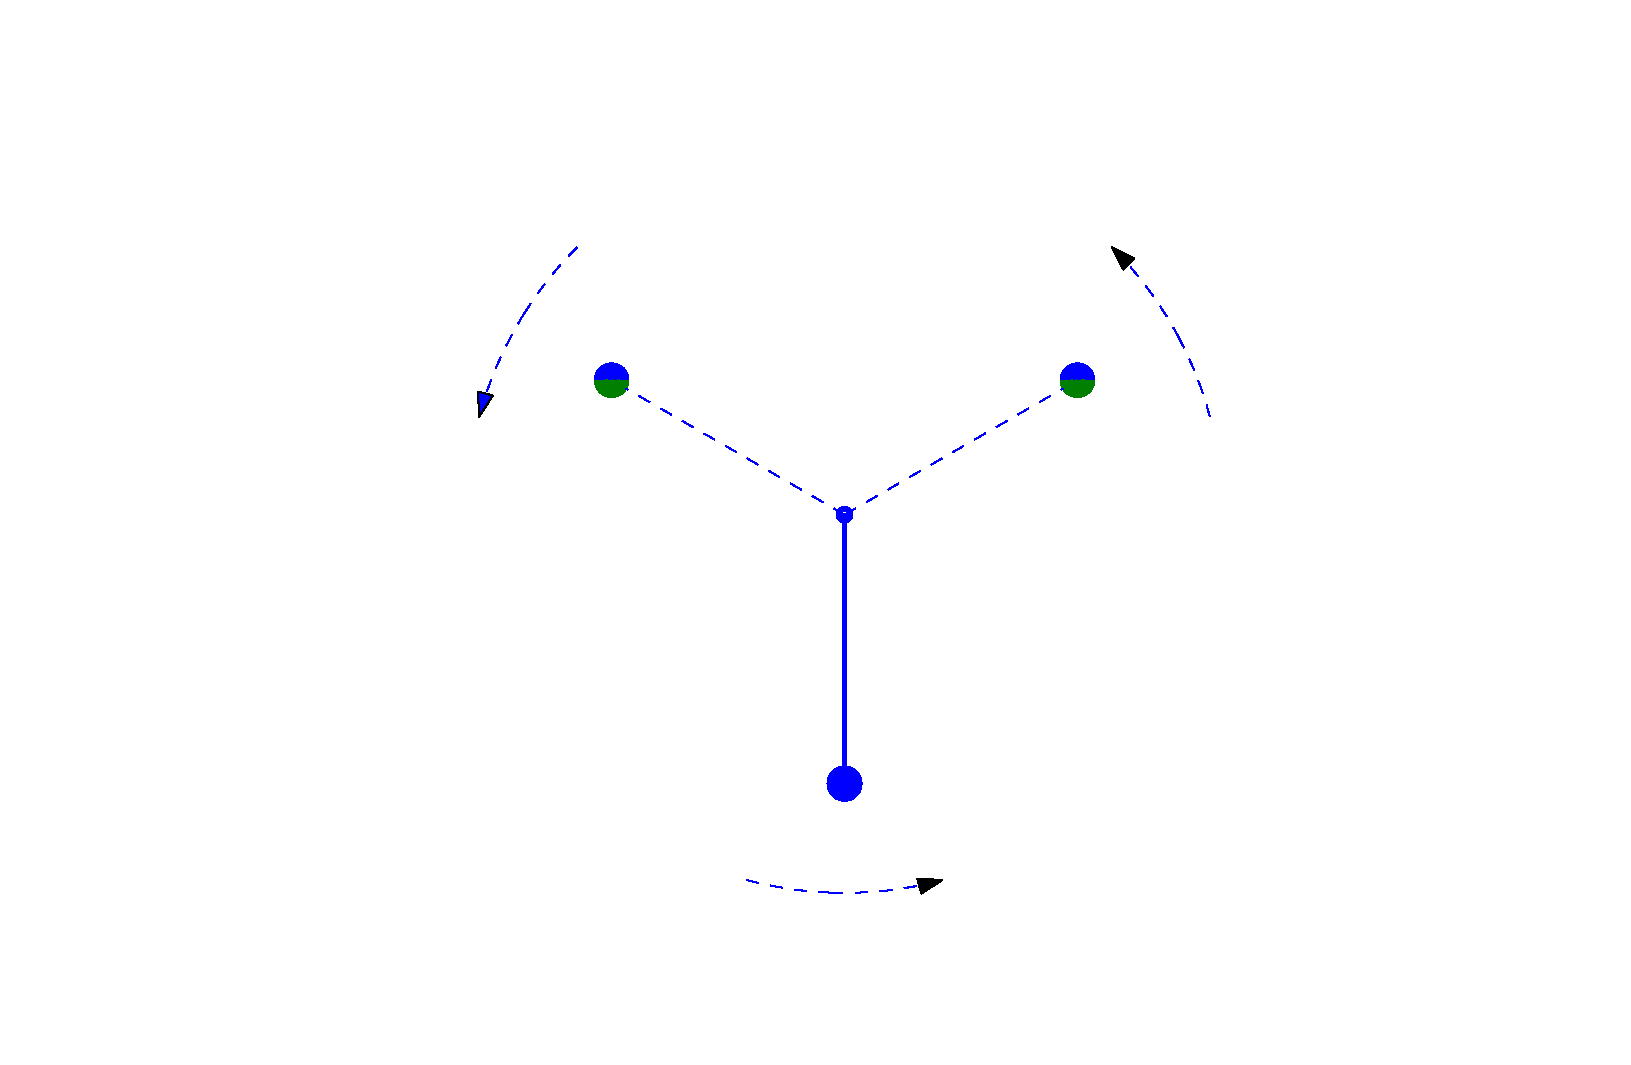
\includegraphics[bb=-78 148 689 643,width=5.67in,height=3.66in,keepaspectratio]{fig040408}}
\caption{The whirling undamped pendulum}
  \label{figure:4.4.8}
  \end{minipage}
  \hspace{0.5cm}
  \begin{minipage}[b]{0.5\linewidth}
    \centering
\scalebox{.7}{
  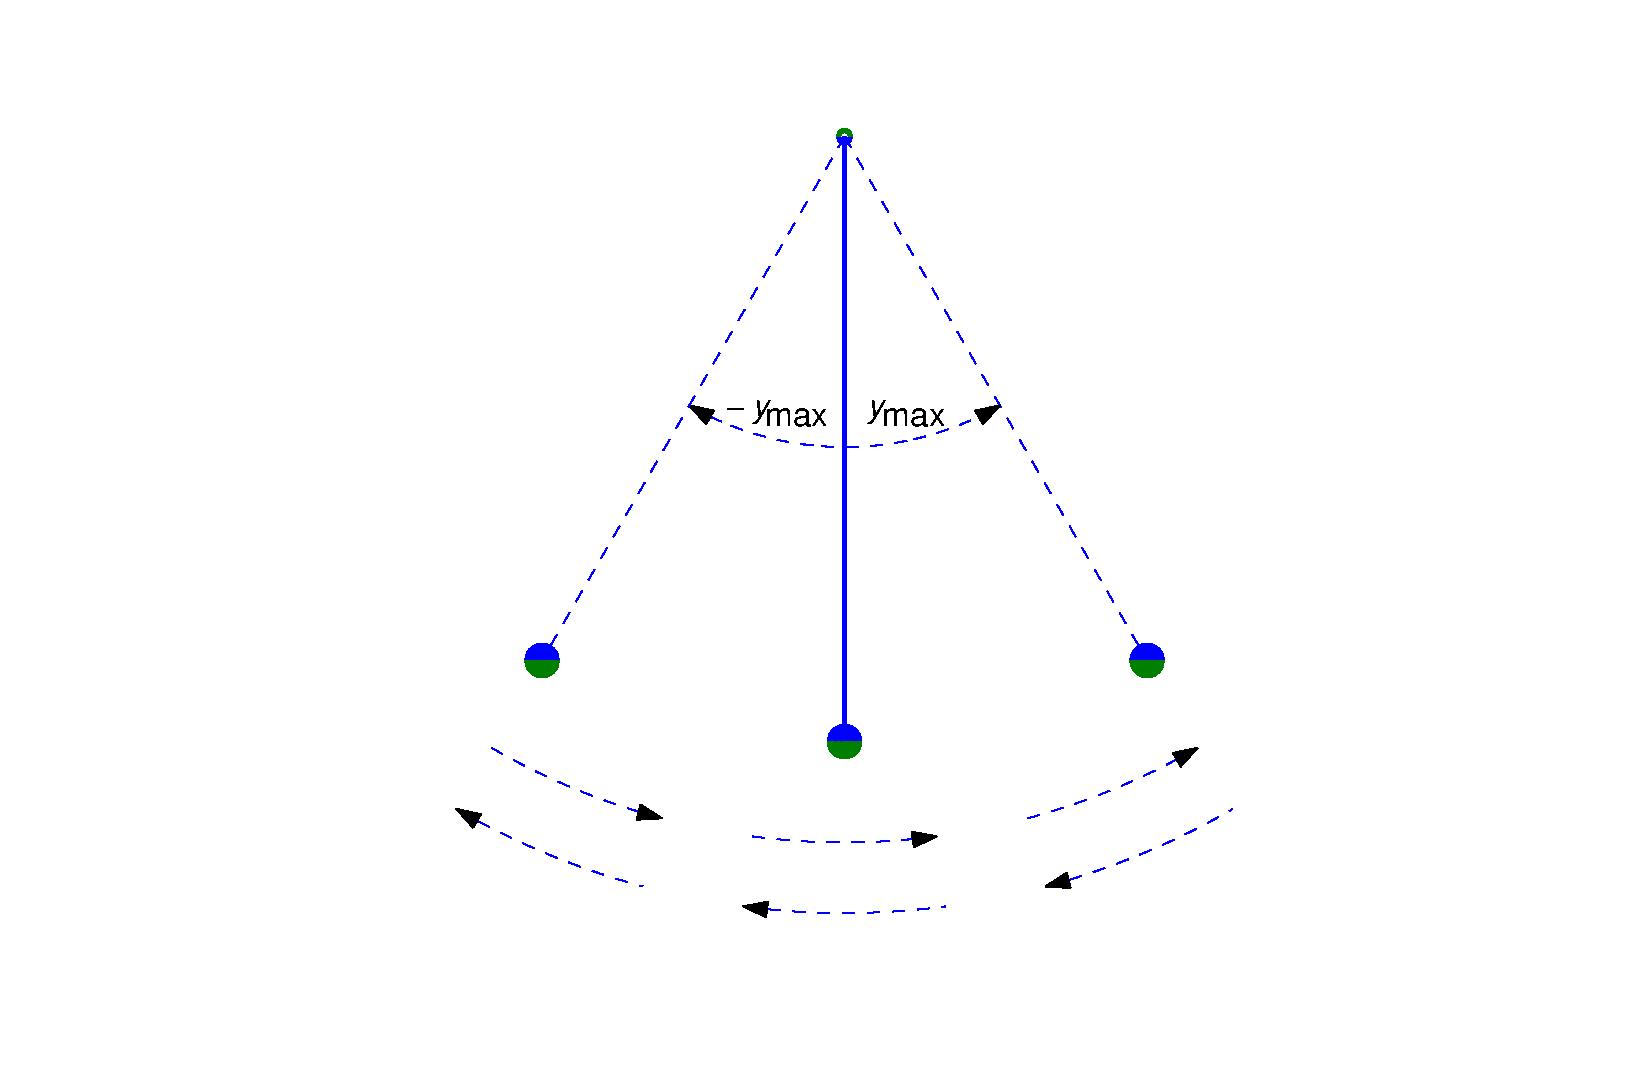
\includegraphics[bb=-78 148 689 643,width=5.67in,height=3.66in,keepaspectratio]{fig040409}}
\caption{ The oscillating undamped pendulum}
  \label{figure:4.4.9}
  \end{minipage}
\end{figure}

\boxit{Stability  and Instability Conditions for $y''+p(y)=0$}

\noindent
It can be shown (Exercise~\ref{exer:4.4.23}) that an equilibrium
$\overline y$ of an undamped equation
\begin{equation} \label{eq:4.4.18}
y''+p(y)=0
\end{equation}
is stable if there's an open interval $(a,b)$ containing $\overline
y$ such that
\begin{equation} \label{eq:4.4.19}
p(y)<0 \mbox{\; if \;}a<y<\overline y\mbox{\; and \;} p(y)>0 \mbox{\; if
\;}
\overline y<y<b.
\end{equation}
If we regard $p(y)$ as a force acting on a unit mass,
\eqref{eq:4.4.19} means that the force resists all sufficiently small
displacements from $\overline y$.

We've already seen examples illustrating this principle. The equation
\eqref{eq:4.4.9} for the undamped spring-mass system is of the form
\eqref{eq:4.4.18} with $p(y)=ky/m$, which has only the stable equilibrium
$\overline y=0$. In this case \eqref{eq:4.4.19} holds with $a=-\infty$ and
$b=\infty$. The equation \eqref{eq:4.4.13} for the undamped pendulum is of
the form \eqref{eq:4.4.18} with $p(y)=(g/L)\sin y$. We've seen that
$\overline y=2m\pi$ is a stable equilibrium if $m$ is an integer. In
this case
$$
p(y)=\sin y<0
\mbox{\; if \;}(2m-1)\pi<y<2m\pi
$$
and
$$
p(y)>0 \mbox{\; if \;}2m\pi<y<(2m+1)\pi.
$$

It can also be shown (Exercise~\ref{exer:4.4.24}) that $\overline y$ is
unstable if there's a $b>\overline y$ such that
\begin{equation} \label{eq:4.4.20}
p(y)<0\mbox{\; if \;}\overline y<y<b
\end{equation}
or an $a<\overline y$ such that
\begin{equation} \label{eq:4.4.21}
p(y)>0\mbox{\; if \;}a<y<\overline y.
\end{equation}
If we regard $p(y)$ as a force acting on a unit mass,
\eqref{eq:4.4.20} means that the force tends to increase all sufficiently
small positive displacements from $\overline y$, while \eqref{eq:4.4.21}
means that the force tends to increase the magnitude of all
sufficiently small negative displacements from $\overline y$.

The undamped pendulum also illustrates this principle. We've seen that
$\overline y=(2m+1)\pi$ is an unstable equilibrium if $m$ is an
integer. In this case
$$
\sin y<0\mbox{\; if \;}(2m+1)\pi<y<(2m+2)\pi,
$$
so \eqref{eq:4.4.20} holds with $b=(2m+2)\pi$, and
$$
\sin y>0\mbox{\; if \;}2m\pi<y<(2m+1)\pi,
$$
so \eqref{eq:4.4.21} holds with $a=2m\pi$.

\begin{example} \label{example:4.4.3}\rm
The equation
\begin{equation} \label{eq:4.4.22}
y''+y(y-1)=0
\end{equation}
is of the form \eqref{eq:4.4.18} with $p(y)=y(y-1)$. Therefore $\overline
y=0$ and $\overline y=1$ are the equilibria of \eqref{eq:4.4.22}. Since
\begin{eqnarray*}
y(y-1)>0 &\text{\, if \,} y<0\mbox{\, or \,}y>1,\\
<0&\hspace*{-22pt}\text{\, if \,} 0<y<1,
\end{eqnarray*}
$\overline y=0$ is unstable and $\overline y=1$ is
stable.

The phase plane equivalent of \eqref{eq:4.4.22} is the separable equation
$$
v{dv\over dy}+y(y-1)=0.
$$
Integrating yields
$$
{v^2\over2}+{y^3\over3}-{y^2\over2}=C,
$$
which we rewrite  as
\begin{equation} \label{eq:4.4.23}
v^2+{1\over3}y^2(2y-3)=c
\end{equation}
after renaming the constant of integration. These are the trajectories
of \eqref{eq:4.4.22}. If $y$ is any solution of \eqref{eq:4.4.22},  the
point $(y(t),v(t))$ moves along the trajectory of $y$ in the direction
of increasing $y$ in the upper half plane ($v=y'>0$), or in the
direction of decreasing $y$ in the lower half plane ($v=y'<0$).

Figure~\ref{figure:4.4.10}  shows
typical trajectories. The
dashed curve through the critical point $(0,0)$, obtained by setting
$c=0$ in \eqref{eq:4.4.23}, separates the $y$-$v$ plane into regions
that contain different kinds of trajectories; again,
 we call this curve a {\color{blue}\it separatrix\/}.
Trajectories in the region bounded by the closed loop \part{b} are closed
curves,
so solutions associated with them are periodic. Solutions associated
with other trajectories are not periodic. If $y$ is any such solution
with trajectory not  on the separatrix, then
$$
\begin{array}{llrllr}
\dst\lim_{t\to\infty}y(t)&=&-\infty, &\dst\lim_{t\to-\infty}y(t)&=&-\infty,\\
\dst\lim_{t\to\infty}v(t)&=&-\infty,
&\dst\lim_{t\to-\infty}v(t)&=&\infty.
\end{array}
$$

 \begin{figure}[H]
  \centering
  \color{blue}
  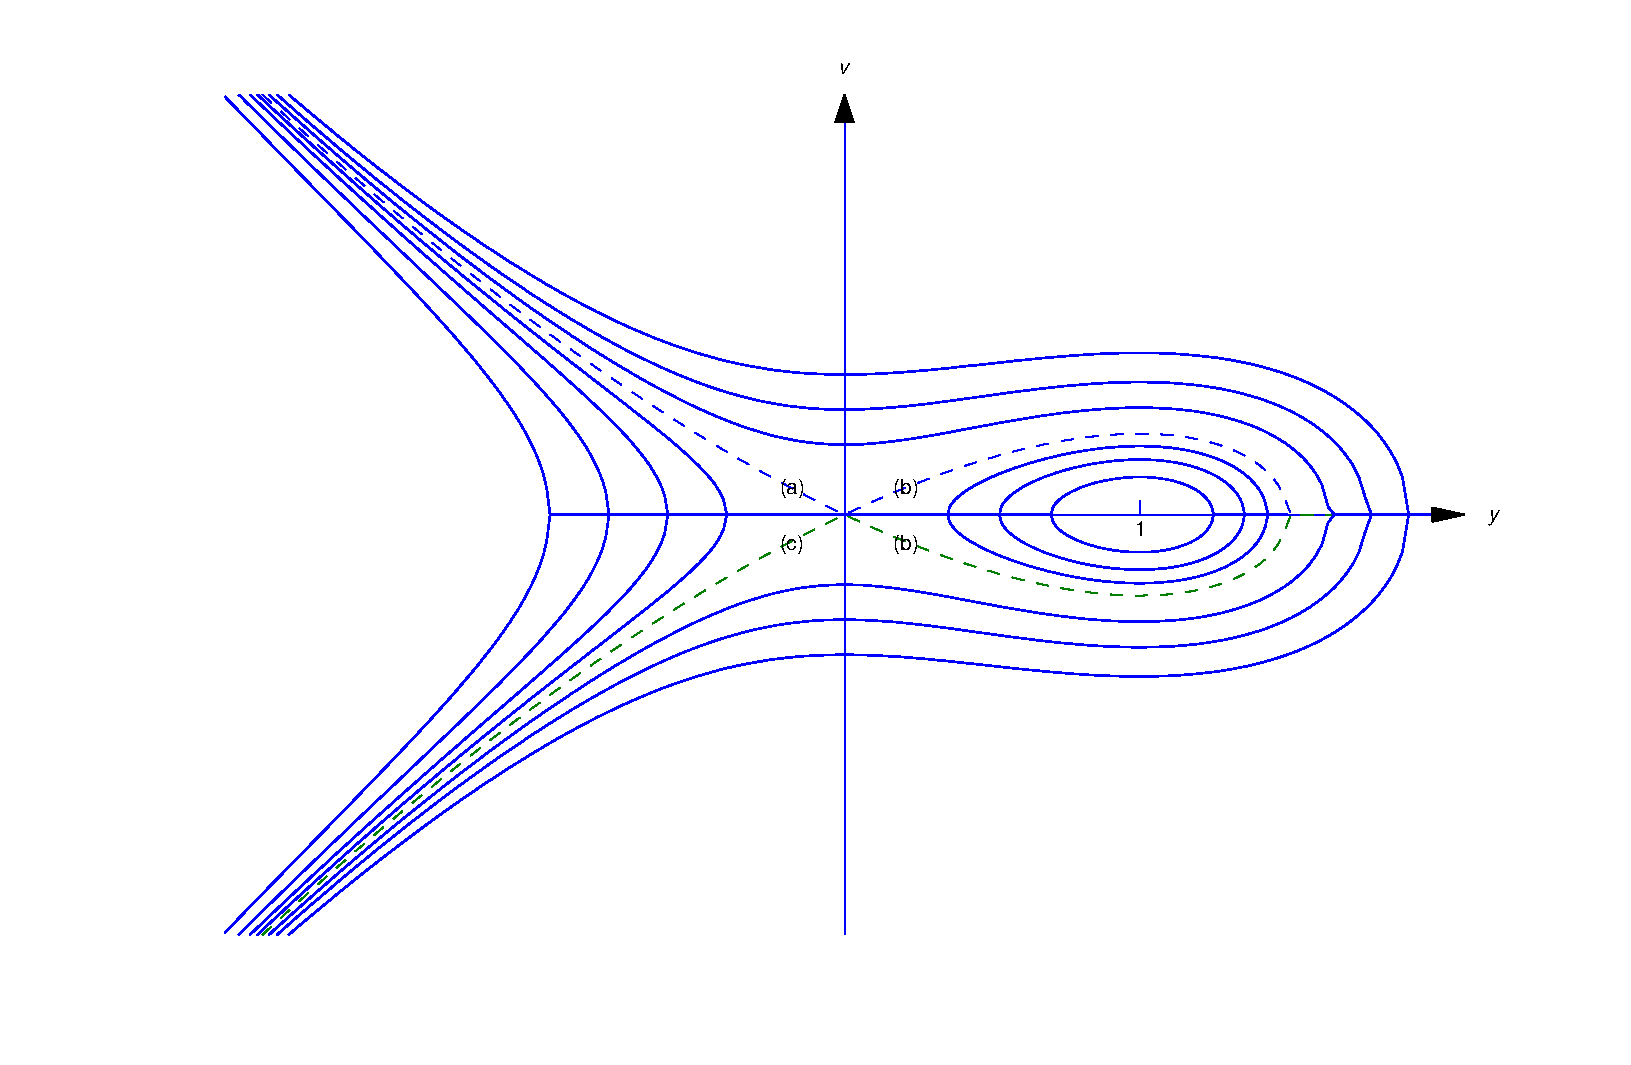
\includegraphics[bb=-78 148 689 643,width=5.67in,height=3.66in,keepaspectratio]{fig040410}
\caption{ Trajectories of $y''+y(y-1)=0$}
  \label{figure:4.4.10}
\end{figure}

The separatrix contains four trajectories of \eqref{eq:4.4.22}. One is the
point $(0,0)$, the trajectory of the equilibrium $\overline y=0$.
Since distinct trajectories can't intersect, the segments of the
separatrix marked \part{a}, \part{b}, and \part{c} -- which don't include $(0,0)$ --
are distinct trajectories, none of which can be traversed in finite
time. Solutions with these trajectories have the following asymptotic
behavior:
$$
\begin{array}{llrllrl}
\dst\lim_{t\to\infty}y(t)&=&0, &\dst\lim_{t\to-\infty}y(t)&=&-\infty,\\
\dst\lim_{t\to\infty}v(t)&=&0,
&\dst\lim_{t\to-\infty}v(t)&=&\infty\phantom{,}&
\mbox{ (on \part{a})}  \\
\dst\lim_{t\to\infty}y(t)&=&0, &\dst\lim_{t\to-\infty}y(t)&=&0,\\
\dst\lim_{t\to\infty}v(t)&=&0,
&\dst\lim_{t\to-\infty}v(t)&=&0\phantom{,}&
\mbox{ (on \part{b})}  \\
\dst\lim_{t\to\infty}y(t)&=&-\infty, &\dst\lim_{t\to-\infty}y(t)&=&0,\\
\dst\lim_{t\to\infty}v(t)&=&-\infty,
&\dst\lim_{t\to-\infty}v(t)&=&0\phantom{,}&
\mbox{ (on \part{c})}.
\end{array}.
$$
\end{example}

\boxit{The Damped Case}

\noindent
The phase plane equivalent of the damped autonomous equation
\begin{equation} \label{eq:4.4.24}
y''+q(y,y')y'+p(y)=0
\end{equation}
is
$$
v{dv\over dy}+q(y,v)v+p(y)=0.
$$
This equation isn't  separable, so we can't solve it for $v$ in terms
of
$y$,
as we did in the undamped case, and conservation of energy doesn't
hold. (For example, energy expended in overcoming friction is lost.)
However, we can study the qualitative behavior of its solutions by
rewriting it as
\begin{equation} \label{eq:4.4.25}
{dv\over dy}=-q(y,v)-{p(y)\over v}
\end{equation}
and considering the direction fields for this equation. In the
following examples we'll also be showing computer generated
trajectories of this equation, obtained by numerical methods. The
exercises call for similar computations. The methods discussed in
Chapter~3
 are not suitable for this
task, since  $p(y)/v$ in \eqref{eq:4.4.25} is undefined on the $y$ axis
of the Poincar\'e phase plane. Therefore we're forced to apply
numerical methods briefly discussed in Section~10.1 to the
system
\begin{eqnarray*}
y'&=&v\\
v'&=&-q(y,v)v-p(y),
\end{eqnarray*}
which is equivalent to \eqref{eq:4.4.24} in the sense defined in
Section~10.1. Fortunately, most differential equation software
packages  enable you to do this painlessly.

In the text we'll confine ourselves to the case where $q$
is constant, so \eqref{eq:4.4.24} and \eqref{eq:4.4.25}  reduce to
\begin{equation} \label{eq:4.4.26}
y''+cy'+p(y)=0
\end{equation}
and
$$
{dv\over dy}=-c-{p(y)\over v}.
$$
(We'll consider more general equations in the exercises.) The constant
$c$ is called the {\color{blue}\it damping constant\/}. In situations where
\eqref{eq:4.4.26} is the equation of motion of an object, $c$ is positive;
however, there are situations where  $c$ may be negative.

\boxit{The Damped Spring-Mass System}

\noindent
Earlier we considered
the spring - mass system under the assumption that the only forces
acting on the object were gravity and the spring's resistance to
changes in its length. Now we'll assume that some mechanism (for
example, friction in the spring or atmospheric resistance) opposes the
motion of the object with a force proportional to its velocity. In
Section~6.1 it will be shown that in this case Newton's
second law of motion implies that
\begin{equation} \label{eq:4.4.27}
my''+cy'+ky=0,
\end{equation}
where $c>0$ is the {\color{blue}\it damping constant\/}. Again, this
equation can
be solved easily by a method that we'll study in Section~5.2,
but that method isn't available here. Instead, we'll consider its
phase plane equivalent, which can be written in the form \eqref{eq:4.4.25}
as
\begin{equation} \label{eq:4.4.28}
{dv\over dy}=-{c\over m}-{ky\over mv}.
\end{equation}
(A minor note: the $c$ in \eqref{eq:4.4.26} actually corresponds to
$c/m$ in this equation.) Figure~\ref{figure:4.4.11} shows a
typical direction field for an equation of this form. Recalling that
motion along a trajectory must be in the direction of increasing $y$
in the upper half plane ($v>0$) and in the direction of decreasing $y$
in the lower half plane ($v<0$), you can infer that all trajectories
approach the origin in clockwise fashion. To confirm this,
Figure~\ref{figure:4.4.12} shows the same direction field with some
trajectories filled in. All the trajectories shown there correspond to
solutions of the initial value problem
$$
my''+cy'+ky=0,\quad y(0)=y_0,\quad y'(0)=v_0,
$$
where
$$
mv_0^2+ky_0^2=\rho\quad (\mbox{a positive constant});
$$
thus, if there were no damping ($c=0$),  all the solutions would
have the same dashed elliptic trajectory, shown in
Figure~\ref{figure:4.4.14}.

\begin{figure}[htbp]
\color{blue}
  \begin{minipage}[b]{0.5\linewidth}
    \centering
   \scalebox{.65}{
  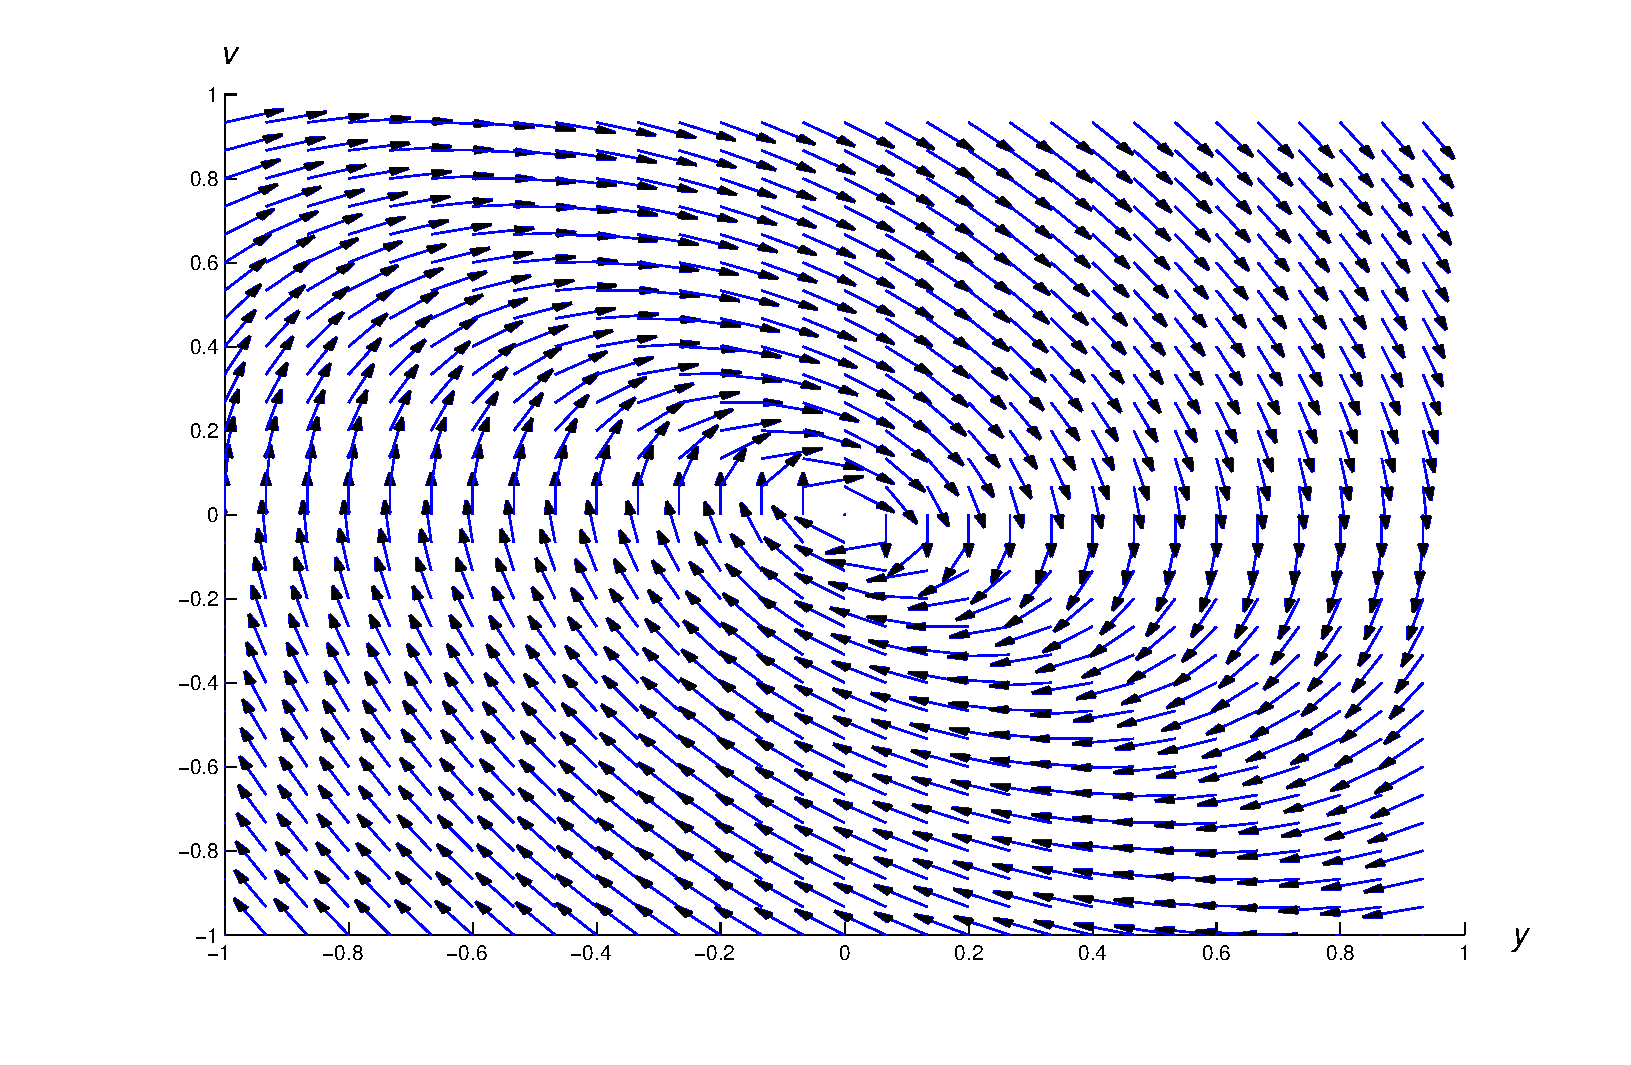
\includegraphics[bb=-78 148 689 643,width=5.67in,height=3.66in,keepaspectratio]{fig040411}}
\caption{ A typical direction field for
$my''+cy'+ky=0$ with $0<c<c_1$}
  \label{figure:4.4.11}
  \end{minipage}
  \hspace{0.6cm}
  \begin{minipage}[b]{0.5\linewidth}
    \centering
   \scalebox{.65}{
  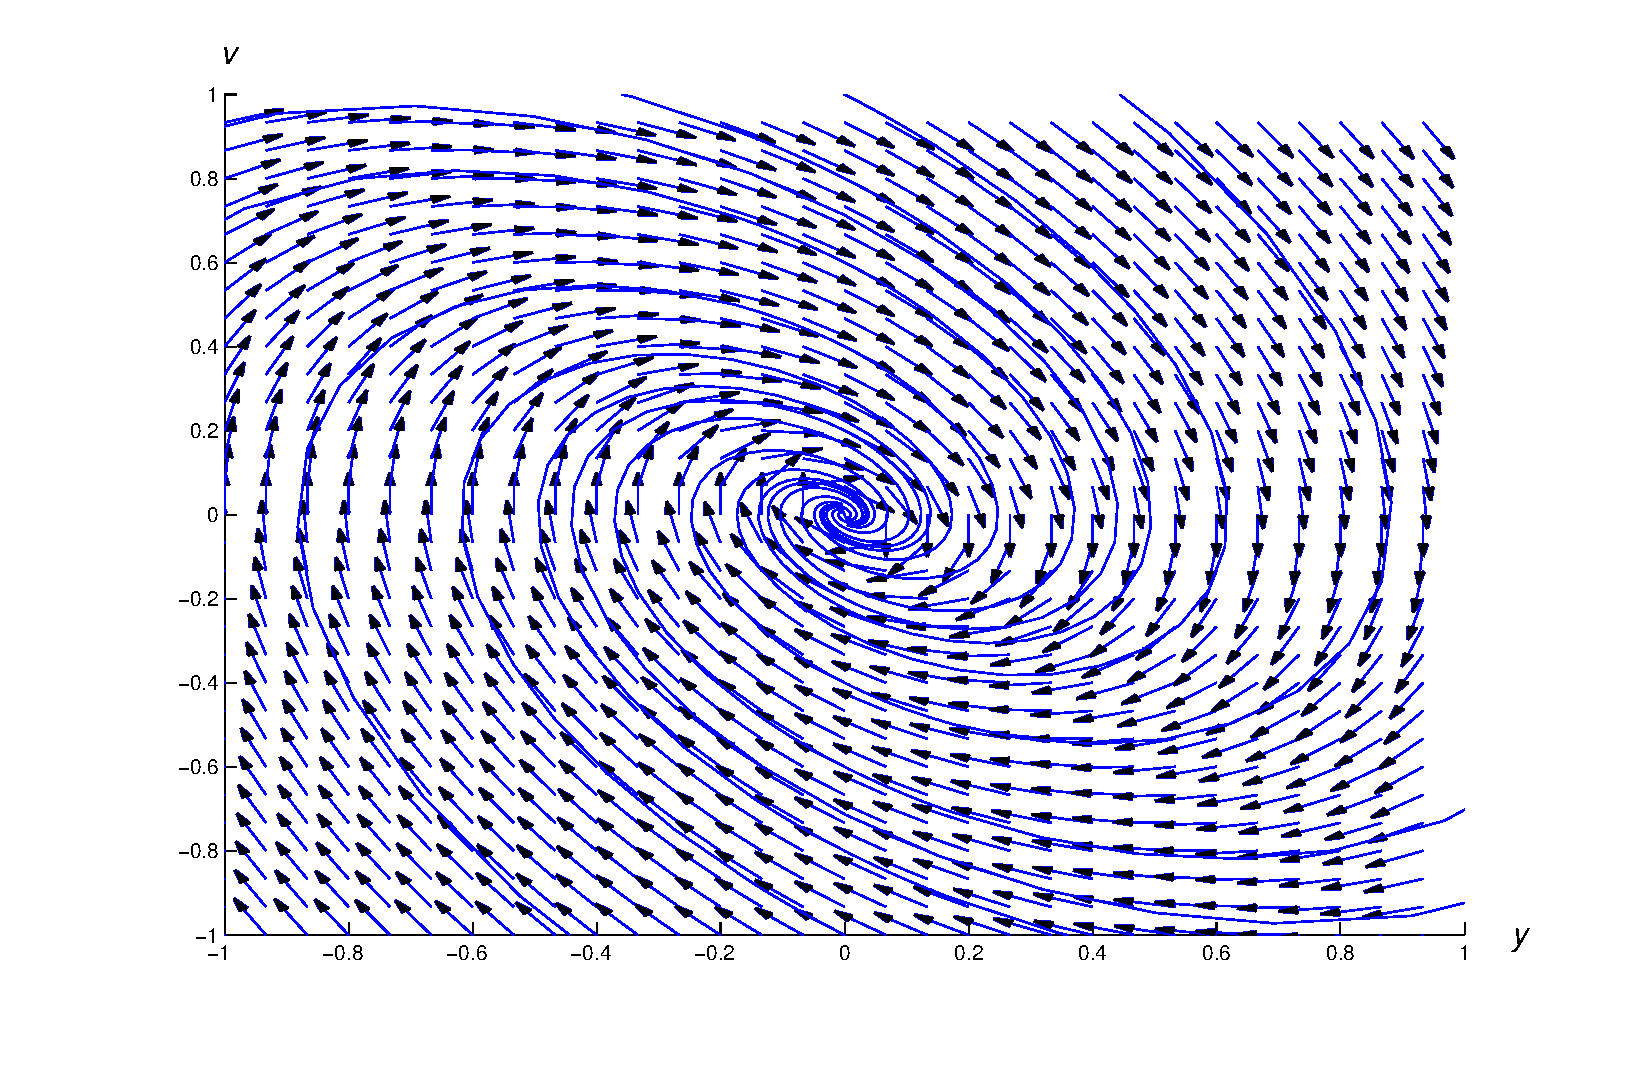
\includegraphics[bb=-78 148 689 643,width=5.67in,height=3.66in,keepaspectratio]{fig040412}}
\caption{ Figure~\ref{figure:4.4.11}
with some trajectories added}
  \label{figure:4.4.12}
  \end{minipage}
\end{figure}

Solutions corresponding to the trajectories in
Figure~\ref{figure:4.4.12} cross the $y$-axis infinitely many times.
The corresponding solutions are said to be {\color{blue}\it
oscillatory\/} (Figure~\ref{figure:4.4.13}) It is shown in
Section~6.2 that there's a number $c_1$ such that if $0\le
c<c_1$ then  all solutions of \eqref{eq:4.4.27} are oscillatory, while if
$c\ge c_1$,  no solutions of \eqref{eq:4.4.27} have this property. (In
fact, no solution not identically zero can have more than two zeros in
this case.) Figure~\ref{figure:4.4.14} shows a direction field and
some integral curves for \eqref{eq:4.4.28} in this case.

\begin{figure}[H]
  \centering
\scalebox{.7}{
  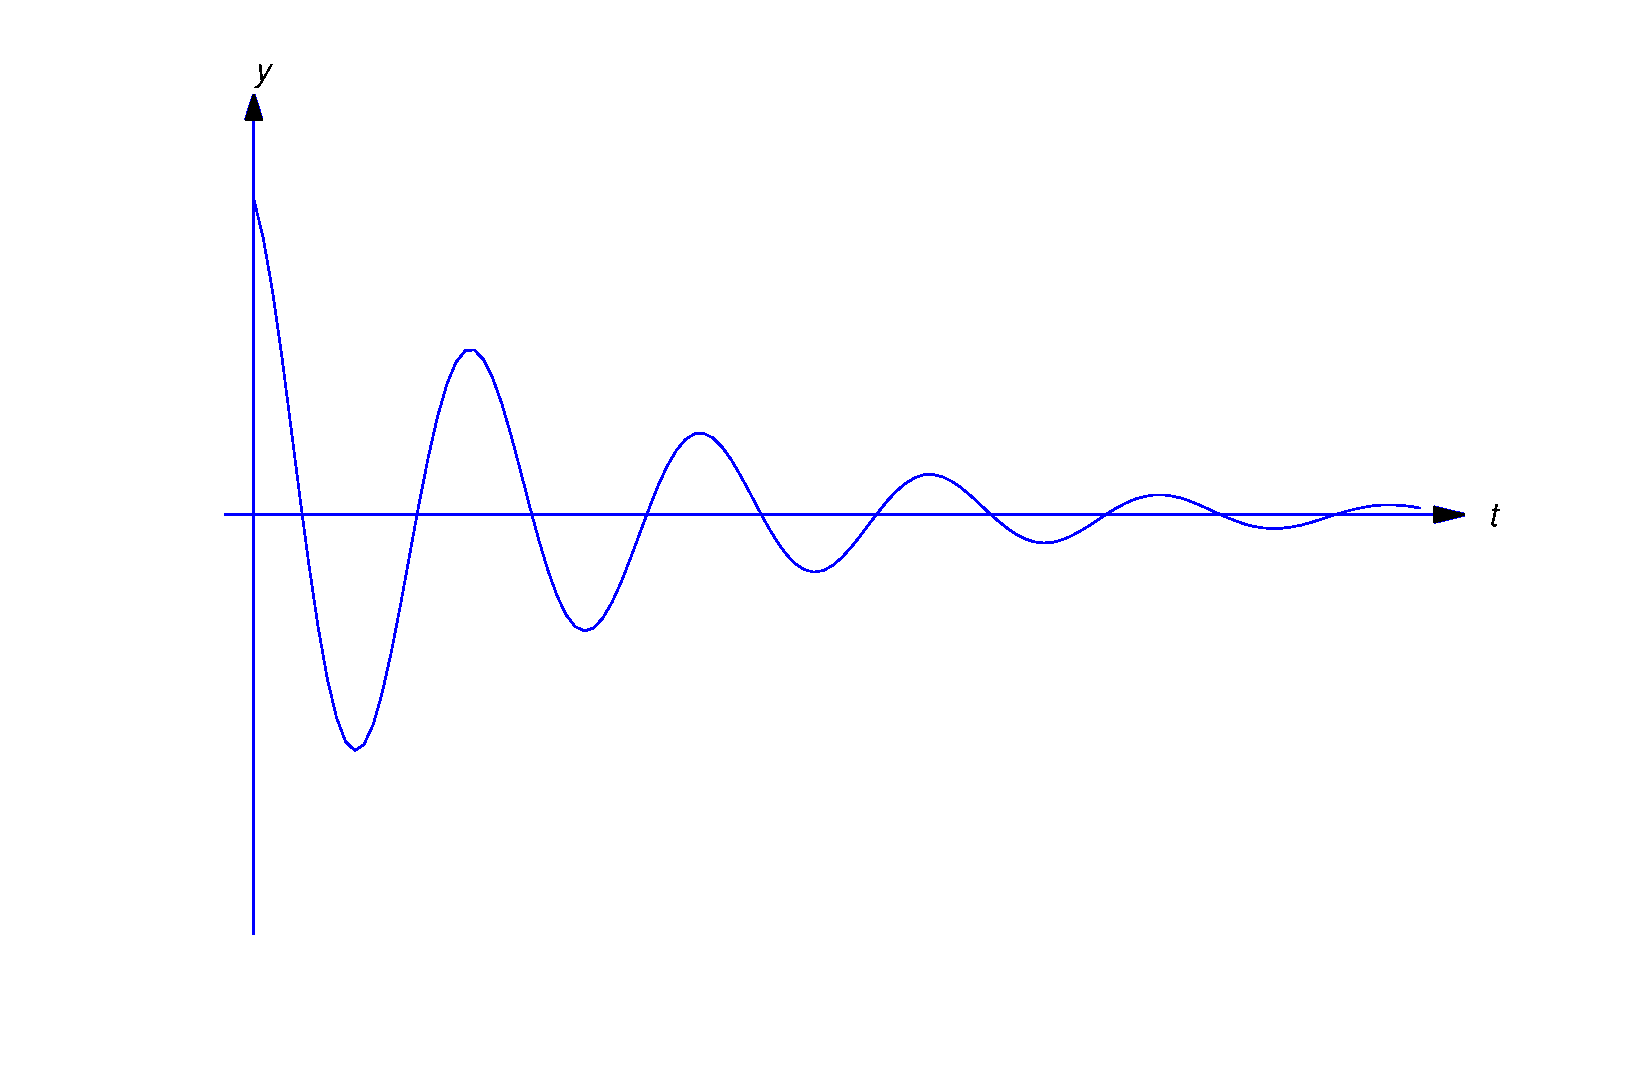
\includegraphics[bb=-78 148 689 643,width=5.67in,height=3.66in,keepaspectratio]{fig040413}}
\color{blue}
\caption{ An oscillatory solution of $my''+cy'+ky=0$}
  \label{figure:4.4.13}
\end{figure}

\begin{example}[The Damped Pendulum]\label{example:4.4.5} \rm
Now we
return to the pendulum. If we assume that
some mechanism (for example, friction in the axle or atmospheric
resistance) opposes the motion of the pendulum with a force
proportional to its angular velocity,  Newton's second law of
motion implies that
\begin{equation} \label{eq:4.4.29}
mLy''=-cy'-mg\sin y,
\end{equation}
where $c>0$ is the damping constant. (Again, a minor note: the $c$
in \eqref{eq:4.4.26} actually corresponds to $c/mL$ in this equation.)
To plot a direction field for \eqref{eq:4.4.29} we write its phase plane
equivalent as
$$
{dv\over dy}=-{c\over mL}-{g\over Lv}\sin y.
$$
Figure~\ref{figure:4.4.15} shows
trajectories of four solutions of \eqref{eq:4.4.29}, all satisfying
$y(0)=0$. For each $m=0$, $1$, $2$, $3$, imparting the initial velocity
$v(0)=v_m$ causes the pendulum to make $m$ complete revolutions and
then settle into decaying oscillation about the stable equilibrium
$\overline y=2m\pi$.
\end{example}

\begin{figure}[H]
  \centering
\scalebox{.8}{
  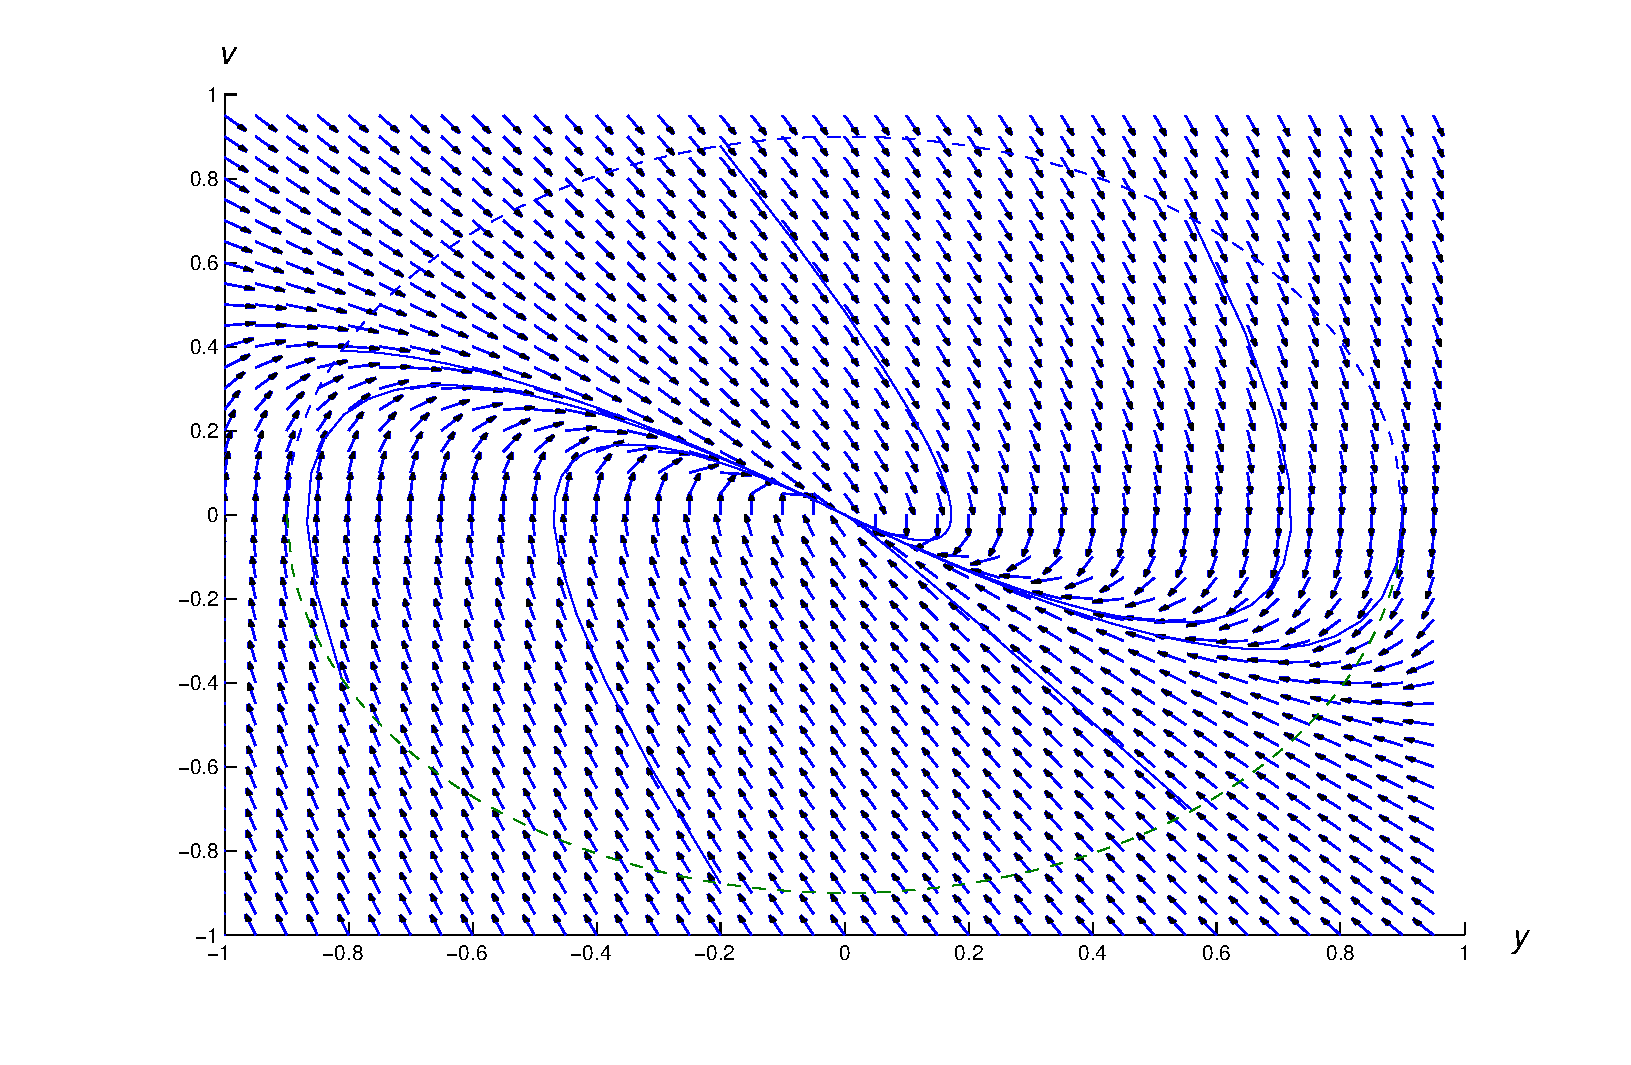
\includegraphics[bb=-78 148 689 643,width=5.67in,height=3.66in,keepaspectratio]{fig040414}}
\color{blue}
\caption{ A typical direction field for
$my''+cy'+ky=0$ with $c>c_1$}
  \label{figure:4.4.14}
\end{figure}

\begin{figure}[H]
  \centering
  \scalebox{.8}{
  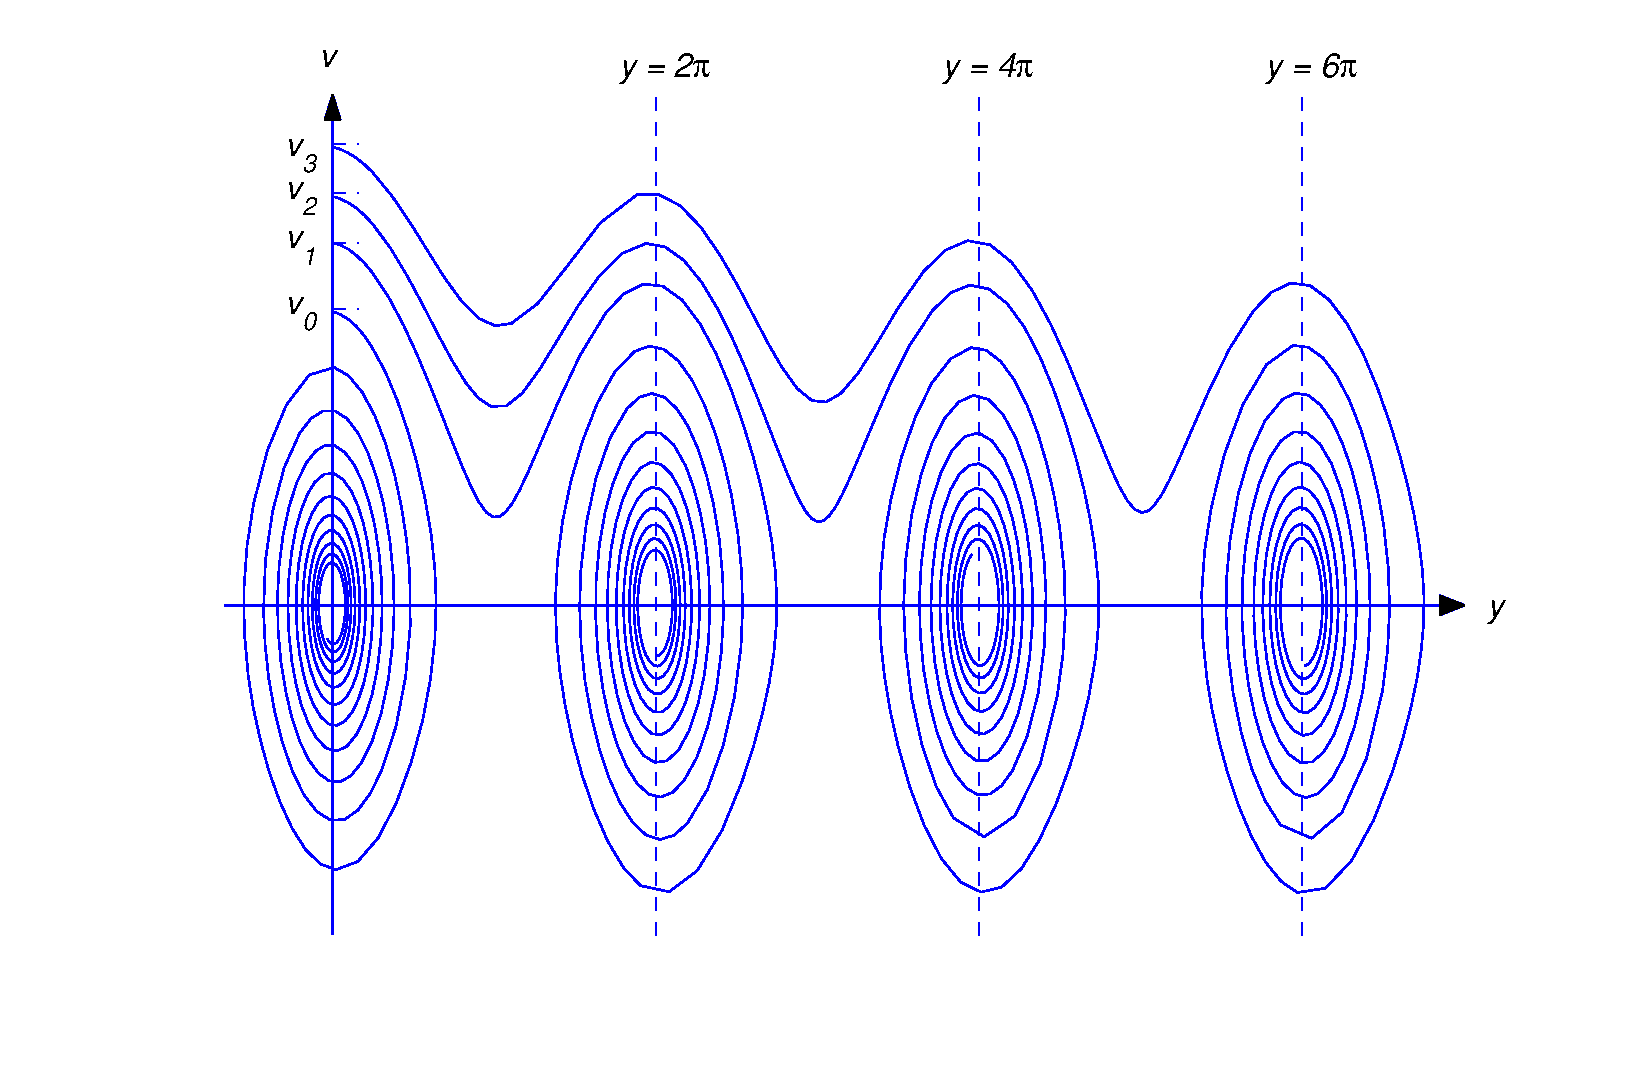
\includegraphics[bb=-78 148 689 643,width=5.67in,height=3.66in,keepaspectratio]{fig040415}}
\color{blue}
\caption{ Four  trajectories of the damped pendulum}
  \label{figure:4.4.15}
\end{figure}

\newpage

\exercises
In Exercises~\ref{exer:4.4.1}--\ref{exer:4.4.4} find the equations of the
trajectories of the given undamped equation. Identify the equilibrium
solutions, determine whether they are stable or unstable, and
plot some trajectories. \hint{Use Eqn.~\eqref{eq:4.4.8} to
obtain the equations of the trajectories.}

\begin{exerciselist}
\begin{tabular}[t]{@{}p{168pt}@{}p{168pt}}
\item\label{exer:4.4.1} \CGex $y''+y^3=0$ &
\vspace*{10pt}\item\label{exer:4.4.2} \CGex $y''+y^2=0$
\end{tabular}

\begin{tabular}[t]{@{}p{168pt}@{}p{168pt}}
\item\label{exer:4.4.3} \CGex$ y''+y|y|=0$ &
\item\label{exer:4.4.4} \CGex $y''+ye^{-y}=0$
\end{tabular}

\exercisetext{
In Exercises~\ref{exer:4.4.5}--\ref{exer:4.4.8} find the equations of the
trajectories of the given undamped equation. Identify the equilibrium
solutions,
determine whether they are stable or unstable, and find the equations
of the separatrices (that is, the curves through the unstable
equilibria). Plot the separatrices and some
trajectories in each of the regions of Poincar\'e plane determined by
them. \hint{Use Eqn.~\eqref{eq:4.4.17} to determine the separatrices.}}

\begin{tabular}[t]{@{}p{168pt}@{}p{168pt}}
\item\label{exer:4.4.5} \CGex $y''-y^3+4y=0$ &
\vspace*{10pt}\item\label{exer:4.4.6} \CGex $y''+y^3-4y=0$
\end{tabular}

%\begin{tabular}[t]{@{}p{168pt}@{}p{168pt}}
\begin{tabular}[t]{@{}p{178pt}@{}p{168pt}}
\item\label{exer:4.4.7} \CGex $y''+y(y^2-1)(y^2-4)=0$&
\item\label{exer:4.4.8} \CGex $y''+y(y-2)(y-1)(y+2)=0$
\end{tabular}

\exercisetext{In Exercises~\ref{exer:4.4.9}--\ref{exer:4.4.12}
plot some trajectories of the given equation for various values
(positive, negative, zero) of the parameter $a$. Find the equilibria
of the equation and classify them as stable or unstable. Explain why
the phase plane plots corresponding to positive and negative values of
$a$ differ so markedly. Can you think of a reason why zero deserves to
be called the {\color{blue}\it critical value\/} of $a$?}

\begin{tabular}[t]{@{}p{168pt}@{}p{168pt}}
\item\label{exer:4.4.9} \Lex $y''+y^2-a=0$&
\vspace*{10pt}\item\label{exer:4.4.10} \Lex $y''+y^3-ay=0$
\end{tabular}

\begin{tabular}[t]{@{}p{168pt}@{}p{168pt}}
\item\label{exer:4.4.11} \Lex $y''-y^3+ay=0$&
\item\label{exer:4.4.12} \Lex $y''+y-ay^3=0$
\end{tabular}
\exercisetext{In Exercises~\ref{exer:4.4.13}-\ref{exer:4.4.18}
plot trajectories of the given equation for $c=0$ and small nonzero
(positive and negative) values of $c$ to observe the effects of
damping.}

\begin{tabular}[t]{@{}p{168pt}@{}p{168pt}}
\item\label{exer:4.4.13} \Lex $y''+cy'+y^3=0$&
\vspace*{10pt}\item\label{exer:4.4.14} \Lex $y''+cy'-y=0$
\end{tabular}

\begin{tabular}[t]{@{}p{168pt}@{}p{168pt}}
\item\label{exer:4.4.15} \Lex $y''+cy'+y^3=0$&
\item\label{exer:4.4.16} \Lex $y''+cy'+y^2=0$
\end{tabular}

\begin{tabular}[t]{@{}p{168pt}@{}p{168pt}}
\item\label{exer:4.4.17} \Lex $y''+cy'+y|y|=0$&
\item\label{exer:4.4.18} \Lex $y''+y(y-1)+cy=0$
\end{tabular}

\item\label{exer:4.4.19} \Lex
The \href{https://mathshistory.st-andrews.ac.uk/Biographies/Van_der_Pol/}
{\color{blue}\it van der Pol equation}
$$
y''-\mu(1-y^2)y'+y=0,
\eqno{\rm(A)}
$$
where $\mu$ is a positive constant and $y$ is electrical current
(Section~6.3), arises in the study of an electrical circuit
whose resistive properties depend upon the current. The damping term \\
$-\mu(1-y^2)y'$ works to reduce $|y|$ if $|y|<1$ or to increase $|y|$
if
$|y|>1$. It can be shown that van der
Pol's equation has exactly one closed trajectory, which is called a
{\color{blue}\it limit cycle\/}. Trajectories inside the limit cycle spiral
outward to it, while trajectories outside the limit cycle spiral
inward to it (Figure~\ref{figure:4.4.16}). Use your favorite
differential equations software  to verify this for
$\mu=.5,1.1.5,2$. Use a grid with $-4<y<4$ and $-4<v<4$.

\begin{figure}[H]
  \centering
  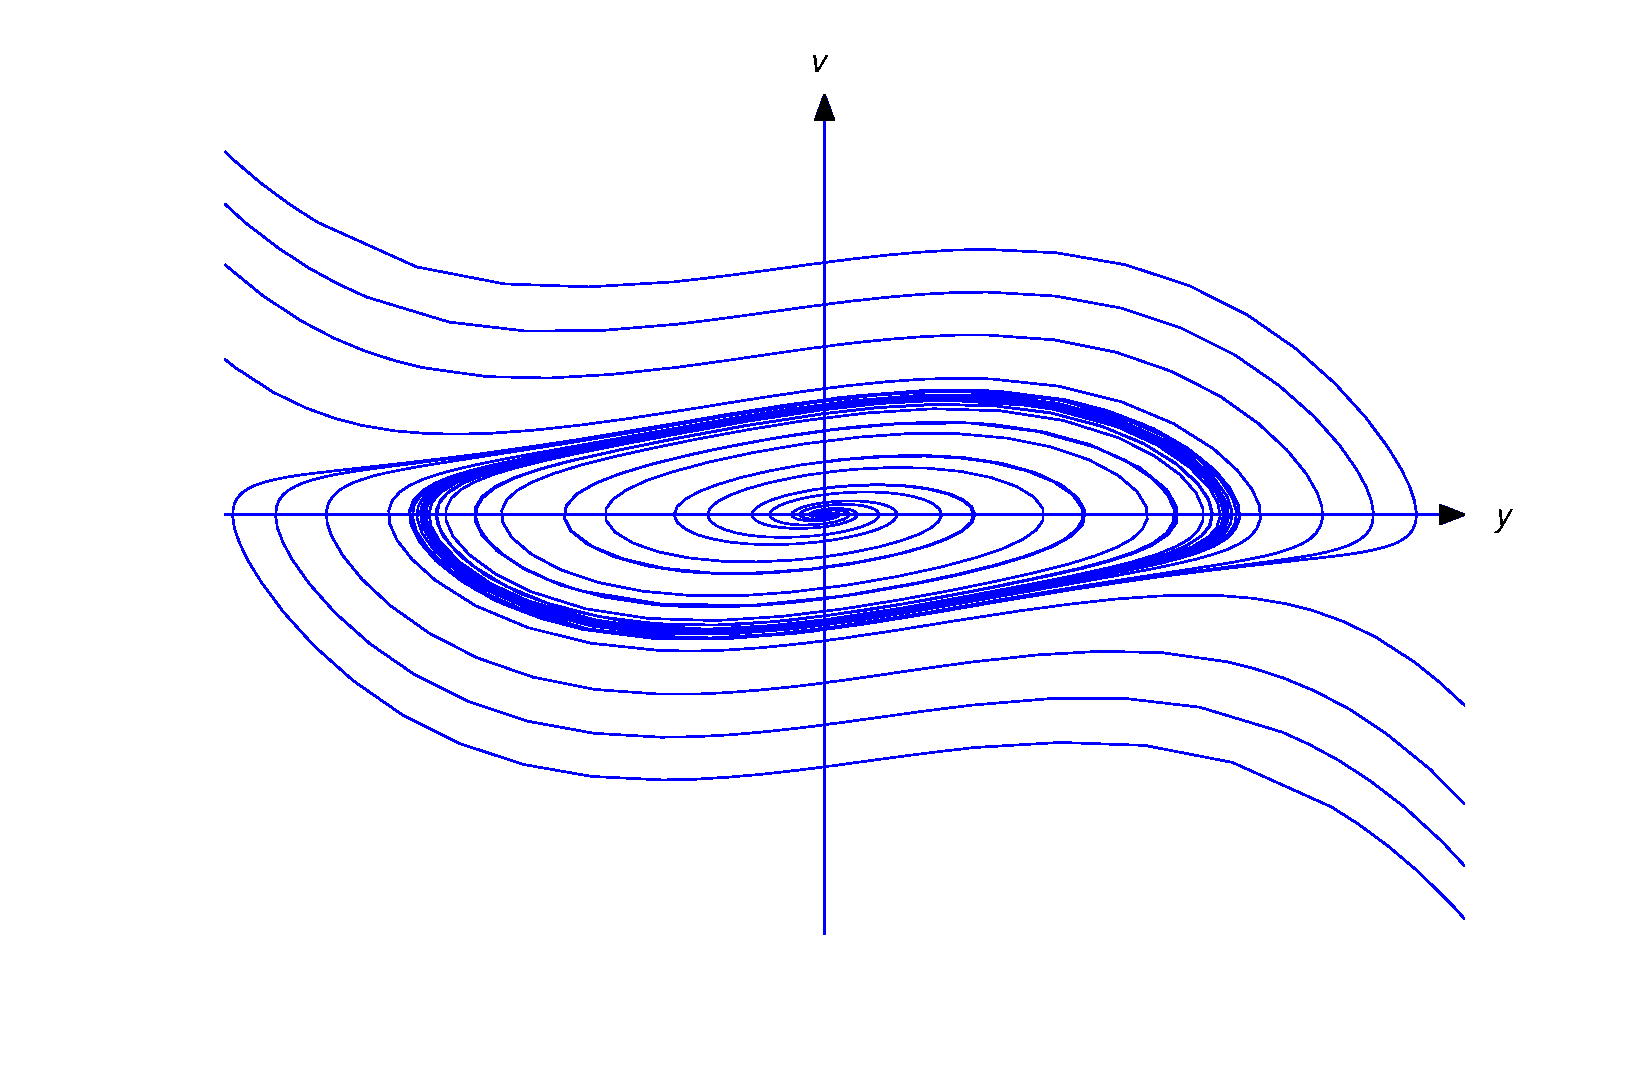
\includegraphics[bb=-78 148 689 643,width=5.67in,height=3.66in,keepaspectratio]{fig040416}
  \caption{Trajectories of van der Pol's equation}
  \label{figure:4.4.16}
\end{figure}

\item\label{exer:4.4.20}  \Lex
\href{https://mathshistory.st-andrews.ac.uk/Biographies/Rayleigh/}
{\color{blue}\it Rayleigh's equation},
$$
y''-\mu(1-(y')^2/3)y'+y=0
$$
also has a limit cycle. Follow the directions of
Exercise~\ref{exer:4.4.19} for this equation.

\item\label{exer:4.4.21}
In connection with Eqn~\eqref{eq:4.4.15},
suppose   $y(0)=0$ and $y'(0)=v_0$, where $0<v_0<v_c$.
\begin{alist}
\item % (a)
Let  $T_1$ be the time
required for  $y$ to increase from zero to
$y_{\max}=2\sin^{-1}(v_0/v_c)$. Show that
$$
{dy\over dt}=\sqrt{v_0^2-v_c^2\sin^2y/2},\quad 0\le t<T_1.
\eqno{\rm(A)}
$$
\item % (b)
Separate variables in (A) and show that
$$
T_1=\int_0^{y_{\max}}{du\over\sqrt{v_0^2-v_c^2\sin^2u/2}}
\eqno{\rm(B)}
$$
\item % (c)
Substitute $\sin u/2=(v_0/v_c)\sin\theta$ in (B) to obtain
$$
T_1=2\int_0^{\pi/2}{d\theta\over\sqrt{v_c^2-v_0^2\sin^2\theta}}.
\eqno{\rm(C)}
$$
\item % (d)
Conclude from  symmetry
that  the time required for  $(y(t),v(t))$ to traverse the
trajectory
$$
v^2=v_0^2-v_c^2\sin^2y/2
$$
is $T=4T_1$, and that consequently $y(t+T)=y(t)$ and $v(t+T)=v(t)$;
that is, the oscillation is periodic with period $T$.
\item % (e)
Show that if $v_0=v_c$,  the integral in (C) is improper and
diverges to $\infty$. Conclude from this  that $y(t)<\pi$
for all $t$ and $\lim_{t\to\infty}y(t)=\pi$.
\end{alist}

\item\label{exer:4.4.22}
Give a direct definition of an unstable equilibrium of $y''+p(y)=0$.

\item\label{exer:4.4.23}
Let $p$ be continuous for all $y$ and $p(0)=0$. Suppose there's
a positive number $\rho$ such that $p(y)>0$ if $0<y\le \rho$ and
$p(y)<0$ if $-\rho\le y<0$. For $0<r\le\rho$ let
$$
\alpha(r)=\min\left\{\int_0^r p(x)\,dx,\ \int_{-r}^0
|p(x)|\,dx\right\}
\mbox{\quad and \quad}
\beta(r)=\max\left\{\int_0^r p(x)\,dx,\ \int_{-r}^0
|p(x)|\,dx\right\}.
$$
Let $y$ be the solution of the initial value problem
$$
y''+p(y)=0,\quad y(0)=v_0,\quad y'(0)=v_0,
$$
and define
$c(y_0,v_0)=v_0^2+2\int_0^{y_0}p(x)\,dx$.
\begin{alist}
\item % (a)
Show that
$$
0<c(y_0,v_0) <v_0^2+2\beta(|y_0|)\mbox{\quad if \quad} 0<|y_0|\le\rho.
$$
\item % (b)
Show that
$$
v^2+2\int_0^y p(x)\,dx=c(y_0,v_0),\quad t>0.
$$
\item % (c)
Conclude from \part{b} that if $c(y_0,v_0)<2\alpha(r)$ then $|y|<r$, $t>0$.
\item % (d)
Given $\epsilon>0$, let  $\delta>0$ be chosen so that
$$
\delta^2+2\beta(\delta)<\max\left\{\epsilon^2/2,2\alpha(\epsilon/\sqrt2)
\right\}.
$$
Show that if $\sqrt{y_0^2+v_0^2}<\delta$ then
$\sqrt{y^2+v^2}<\epsilon$ for $t>0$, which implies that $\overline
  y=0$ is a stable equilibrium of $y''+p(y)=0$.
\item % (e)
Now let $p$
be continuous for all $y$ and $p(\overline y)=0$, where $\overline y$
is not necessarily zero. Suppose there's a positive number
$\rho$ such that $p(y)>0$ if $\overline y<y\le \overline y+\rho$ and
$p(y)<0$ if $\overline y-\rho\le y<\overline y$. Show that $\overline
y$ is a stable equilibrium of $y''+p(y)=0$.
\end{alist}

\item\label{exer:4.4.24}
Let $p$ be continuous for all $y$.
\begin{alist}
\item % (a)
Suppose $p(0)=0$ and there's a positive number $\rho$ such that
$p(y)<0$ if  $0<y\le \rho$. Let $\epsilon$ be any
number such that
$0<\epsilon<\rho$.
Show that if $y$ is the solution of the initial value problem
$$
y''+p(y)=0,\quad y(0)=y_0,\quad y'(0)=0
$$
with $0<y_0<\epsilon$, then
$y(t)\ge\epsilon$ for some
$t>0$. Conclude that $\overline y=0$ is an unstable equilibrium of
$y''+p(y)=0$. \hint{Let $k=\min_{y_0\le
x\le\epsilon}\left(-p(x)\right)$,
which is positive. Show that if $y(t)<\epsilon$ for $0\le t<T$ then
$kT^2<2(\epsilon-y_0)$.}
\item % (b)
Now let $p(\overline y)=0$, where $\overline y$ isn't  necessarily
zero. Suppose there's a positive number $\rho$ such that
$p(y)<0$ if $\overline y<y\le \overline y+\rho$. Show that $\overline
y$ is an unstable equilibrium of $y''+p(y)=0$.
\item % (c)
Modify your proofs of \part{a} and \part{b} to show that if there's a
positive
number $\rho$ such that $p(y)>0$ if $\overline y-\rho\le y<\overline
y$, then $\overline y$ is an unstable equilibrium of $y''+p(y)=0$.
\end{alist}

\end{exerciselist}
